\chapter{Analýza}
\label{analysis-and-its-results}

Po preskúmaní možností pre vykonanie podrobnej analýzy nasadenia NEL som podľa vypracovaného návrhu implementoval potrebné nástroje.
Úlohou týchto nástrojov je dopracovať sa k stanoveným cieľom mojej práce.  
Najskôr v tejto kapitole popisujem svoju prácu z hľadiska toho, čo bolo implementované.
Potom v sekcií \ref{sec:results} prezentujem jej celkové výsledky.


\section{Implementácia nástrojov pre analýzu}

Potrebné nástroje podľa návrhu práce (viď kapitolu \ref{possible-analysis-strategies}) predstavujú implementované skripty pre dve rozdielne metódy analýzy:
\begin{enumerate}
    \item Práca s HTTP Archive:
    \begin{itemize}
        \item[(a)] získať \textit{historické} dáta, 
        \item analyzovať ich a vyprodukovať výsledné metriky,
        \item výsledky podľa potreby vhodne vizualizovať.
    \end{itemize}

    \item Automatizované prehliadanie súčasného webu:
    \begin{itemize}
        \item[(b)] získať \textit{súčasné} dáta,
        \item analyzovať ich a vyprodukovať výsledné metriky, 
        \item výsledky podľa potreby vhodne vizualizovať.
    \end{itemize}
\end{enumerate}

Skutočnosť, že sa tieto dve metódy odlišujú iba v spôsobe získavania vstupných dát (získavanie dát v prvom kroku) som využil pri návrhu skriptov.
Na začiatok som teda definoval štruktúru výstupných dát z prvého kroku oboch metód.
Spoločná štruktúra dát umožňuje implementovať zvyšné dva kroky pre obe metódy rovnako.
Tabuľka \ref{tab:analysis-data-structure} v prílohách túto štruktúru popisuje. 
% Bližšie ju popisuje nasledujúca sekcia o implementácií nástroja pre HTTP Archive.

\subsection{Skript pre prácu s HTTP Archive}
\label{query_and_store}

Vzhľadom na to, že som sa rozhodol ako primárny zdroj dát použiť projekt HTTP Archive, začal som s implementáciou skriptu pre prácu práve s ním.
K vývoju som pristupoval tak, aby bolo možné dáta sťahovať postupne po jednotlivých mesiacoch. 
Cieľom bolo v ďalších krokoch umožniť postupné vyhodnocovanie výsledných metrík. 
Stratégiu postupného vyhodnocovania metrík som si zvolil z toho dôvodu, že som najskôr potreboval dôkladne otestovať optimalizácie získavania dát spomínané v návrhu práce.
Preto som v prvom rade začal sťahovať a vyhodnocovať iba čiastkové výsledky z malého objemu dát, teda niekoľkých mesiacov na začiatku skúmaného časového obdobia.
Jednorazové stiahnutie všetkých dát by totiž viedlo k spotrebovaniu prevažnej väčšiny dostupných finančných zdrojov pre prácu s historickými dátami.

Tieto prvé testy som vykonával pomocou skriptu prebratého od autorov predošlej analýzy (viď existujúcu analýzu v rámci návrhu v kapitole \ref{possible-analysis-strategies}).
Pri ich vykonávaní som objavil problémy v použití prebratého skriptu týkajúce sa mojej optimalizácie použitého príkazu GoogleSQL na extrahovanie dát.
Cieľom optimalizácie bolo rozšíriť vzorku dát pre každú skúmanú doménu.
Dôsledkom toho, že sa príkaz optimalizovať podarilo, sa objem dát na stiahnutie z BigQuery niekoľkokrát zvýšil.
Prebratý skript však používal knižnicu, ktorá nepodporovala sťahovanie dát s vysokým objemom.
To ma viedlo k vytvoreniu nového skriptu, ktorý sa týmto novým podmienkam prispôsobí.

\subsubsection{Špecifikácia}

Pôvodný, prebratý skript pre sťahovanie dát bol napísaný v jazyku Python3.
Keďže mojím cieľom bolo implementovať rovnakú funkcionalitu, no podporovať veľký objem dát, rozhodol som sa pre implementáciu v rovnakom jazyku.
Nový skript, \code{query\_and\_store.py} som napísal v jazyku Python3 s verziou \code{3.12.0}.
Pôvodný algoritmus bol spustiť GoogleSQL príkaz na BigQuery a stiahnuť jeho službou dočasne uložené výsledky.
Nedostal som sa k informácií o maximálnej veľkosti dočasných výsledkov, no z pozorovania som zistil, že zlyhávajú pokusy stiahnuť viac ako 100 megabajtov dát.
Zistil som, že vhodnou alternatívou k tomuto prístupu je vyexportovať výsledné dáta do úložiska Google Cloud Storage nazvaného \textit{bucket} (ďalej už len GCS a GCS bucket).
Pre službu GCS existuje knižnica \code{google.cloud.storage}, ktorá implementuje klienta pre operácie ako práve sťahovanie veľkých objemov dát z GCS bucketov.
Pomocou pôvodnej knižnice, \code{google.cloud.bigquery}, som implementoval rozhranie pre extrahovanie a export dát z BigQuery.
Za pomoci novej knižnice som implementoval rozhranie pre sťahovanie dát z GCS.

Výstupom pôvodného skriptu boli komprimované súbory Apache Parquet, ktoré rovnako ako BigQuery ukladajú dáta formátované s orientáciou na stĺpce.
Keďže použitím nového skriptu výrazne narastá objem analyzovaných dát, schopnosť vyberať iba niektoré potrebné stĺpce pre výpočty konkrétnej metriky je kľúčová z hľadiska pamäťovej náročnosti.
Rozhodol som sa preto ponechať pôvodný formát výstupov aj pre nový skript. 
Na základe toho, že HTTP Archive uverejňuje svoje výsledky po mesiacoch, sú celkovým výstupom 
nového skriptu všetky relevantné informácie o zdrojoch za daný mesiac.
Tieto relevantné informácie sú definované ako polia v tabuľke \ref{tab:analysis-data-structure} v prílohách.
Množinu mesiacov, pre ktoré sa majú stiahnuť dáta, je možné definovať v konfigurácií skriptu.
Výstupné dáta tohto skriptu slúžia pre analýzu metrík nasadenia NEL.
Dáta štruktúrované podľa vyššie uvedenej tabuľky teda filtrujem na len tie zdroje, ktoré sú korektne monitorované technológiou NEL.
Pre nemonitorované alebo nekorektne monitorované (nesprávna konfigurácia) zdroje a domény, si však zaznamenávam ich celkové počty.

\subsubsection{Problémy}

Mesačné dáta HTTP Archive sa v BigQuery vyskytujú rozdelené do dvoch tabuliek (bližšie informácie o rozdelení v sekcií \ref{big-query}):
\begin{enumerate}
    \item tabuľka s dátami z prostredia \code{desktop}, napríklad: \code{2018\_09\_01\_desktop},
    \item tabuľka s dátami z prostredia \code{mobile}, napríklad: \code{2018\_09\_01\_mobile}.
\end{enumerate}

Po konzultácií s pánom Polčákom som zistil, že v predchádzajúcej analýze pracovali s týmto rozdelením tak, že obsah tabuliek zlúčili \cite{nel-http-archive}.
Bolo to však robené manuálne, pretože spracovávali vcelku iba 6 mesiacov.
Keďže je počet skúmaných mesiacov v tejto práci oveľa vyšší, rozhodol som sa zlúčenie automatizovať.
Riešenie som zapracoval do použitého príkazu GoogleSQL.

Ďalej, okrem vyššie spomenutého rozdelenia mesačných dát sa v vyskytovali aj mesiace, ktoré boli rozdelené na časti, napríklad:
\begin{enumerate}
    \item \code{2018\_09\_01\_desktop},
    \item \code{2018\_09\_01\_mobile},
    \item \code{2018\_09\_15\_desktop},
    \item \code{2018\_09\_15\_mobile}.
\end{enumerate}

Tento problém som rovnako vyriešil postupným zlučovaním dát z jednotlivých čiastkových tabuliek v príkaze GoogleSQL.
V oboch spomínaných problémoch som rátal s duplicitami dát a preferoval som výber jedinečných záznamov z neskoršieho dátumu za daný mesiac a záznamy z tabuliek \code{desktop} pred tými z tabuliek \code{mobile}.

% TODO priklad pouzitia na obrázku

\subsection{Skript pre automatizované prehliadanie súčasného webu}
\label{crawl_and_store}

Automatizovaný prehliadač súčasného webu implementuje skript \code{crawl\_and\_store.py}.
Je implementovaný pomocou jazyka Python3 vo verzií \code{3.12.0}. Z knižníc automatizujúcich webový 
prehliadač (viď sekciu \ref{selenium}) som si vybral \textit{Playwright}. 
Za pomoci jej rozhrania prehliadam webové stránky na doménach patriacich do zoznamu domén preskúmaných v najaktuálnejších mesačných dátach z HTTP Archive.
Zoznam týchto domén je však možné spravovať pomocou vedľajšieho skriptu \code{select\_domains\_to\_crawl.ipynb}.
Práve jeho úlohou je načítať celkový zoznam domén, vybrať z nich tie, ktoré majú byť preskúmané a uložiť ich do súboru, ktorý hlavný skript pri spustení použije ako vstup.

Pre každú doménu si najskôr vyžiada domovskú stránku a v prípade úspešnej odpovede z jej obsahu extrahuje všetky dostupné hyperlinky smerujúce na tú istú doménu.
Extrahované hyperlinky udržuje v pomocných objektoch triedy \code{DomainLinkTree}.
Ide o implementáciu stromovej štruktúry pre zoznam dostupných hyperlinkov smerujúcich na aktuálne skúmanú doménu. 
Pri prehliadaní danej domény sa tento strom prehľadáva do šírky (\textit{breadth first search}) aby bol nájdený ďalší hyperlink, ktorý ešte skript nenavštívil.
Najskôr sa teda prehliadajú rozdielne odvetvia stránok (\code{'/home/x'}, \code{'/login/y'}, \code{'/news/z'}) a až potom rôzne zdroje v nich obsiahnuté (\code{'/home/x'}, \code{'/home/y'}, \code{'/home/z'}).
Táto stratégia je doplnená o limitovanie maximálneho počtu hyperlinkov, ktoré má skript preskúmať.
Cieľom takejto implementácie je získať prehľad o využití NEL monitorovania v čo najviac odvetviach stránok na doméne.
Som si však vedomý, že táto stratégia sa nedá uplatniť pre domény, ktoré neštruktúrujú cesty k svojim stránkam do takýchto odvetví --- majú jednoúrovňové cesty k zdrojom.
V takých prípadoch generuje \code{DomainLinkTree} ďalšie hyperlinky podľa poradia, v akom sú pridávané.

Potrebné dáta sa získavajú z hlavičiek v HTTP odpovediach z prehliadaných stránok, ale aj z nimi používaných zdrojov ako sú obrázky, skripty a iné.
Tieto dáta sú pre každú doménu separátne ukladané do registra \code{DomainNelDataRegistry}.
Uvedený register predstavuje objekt triedy implementujúcej rozhranie pre prácu so získanými dátami. 
Na pozadí používa \code{DataFrame} objekty z Python knižnice \textit{pandas}, do ktorých dáta priebežne pridáva.
Po dokončení prehliadania každej domény sa z nej získané dáta v registri ukladajú na disk ako Apache Parquet súbory.
Po dokončení prehliadania poslednej domény sa všetky vytvorené Parquet súbory zlúčia do jedného.
To je docielené tak, že sa všetky načítajú do pamäte skriptu, prepočítajú sa celkové počty spracovaných domén a zdrojov a výsledok sa uloží na disk v štruktúre zdieľanej s HTTP Archive skriptom, popísanej tabuľkou \ref{tab:analysis-data-structure}.

\subsection{Skripty pre analýzu a produkovanie výsledných metrík}
\label{analyze_results}

Po úspešnom behu jedného z predošlých skriptov musia byť ako vstupy do tohto kroku dostupné dáta obsahujúce získané informácie o stave používania NEL na skúmaných doménach.
Z týchto vstupov skripty \code{analyze\_httparchive.py} a \code{analyze\_crawled.py} produkujú predom definované metriky (viď návrh v kapitole \ref{possible-analysis-strategies}).
Uvedené dva skripty sú z pohľadu funkcionality rovnaké, no rozhodol som ich nezlúčiť pre jednoduchosť práce pri opakovanom vykonávaní analýzy vo fáze testovania.
Líšia sa totiž v tom, odkiaľ dáta čerpajú a kam dáta zapisujú.

Oba analyzačné skripty vnútorne používajú rovnakú knižnicu určenú pre spracovanie dát do spomínaných výsledných metrík.
Túto knižnicu, \code{nel\_analysis.py}, som implementoval pomocou \textit{pandas}, knižnice tretej strany pre dátovú analýzu.
Analyzačné skripty vstupné dáta pre každý skúmaný mesiac načítajú, funkcie knižnice vypočítajú výsledky a uložia ich na nové miesto na disku tak, aby sa vstupy zachovali.
Výstupy tohto kroku teda predstavujú zanalyzované dáta, teda výsledky analýzy v ich plnom rozsahu.

\subsubsection{Využitie zoznamov Public Suffix List}

Mnou implementovaná knižnica \code{nel\_analysis.py} okrem \textit{pandas} používa aj ďalšiu prevzatú knižnicu -- \textit{publicsuffix2}\footnote{\href{https://pypi.org/project/publicsuffix2/}{https://pypi.org/project/publicsuffix2/}}.
V prípadoch, keď je pre výpočet metriky potrebné zistiť registrovateľnú časť celkového doménového mena,
sú na to použité funkcie tejto knižnice pracujúce so zoznamom Public Suffix List (PSL). Príkladom použitia je získavanie registrovateľných častí domén prislúchajúcim NEL kolektorom pre identifikáciu ich poskytovateľa.

Je možnosť využiť funkcie tejto knižnice, ktoré interne používajú aktuálny PSL.
Ja ale používam ňou implementovanú funkciu umožňujúcu zvoliť si vlastný PSL.
PSL zoznamy, ktoré som sa rozhodol použiť, som manuálne stiahol z repozitára GitHub, v rámci ktorého je oficiálny projekt PSL verziovaný\footnote{\href{https://github.com/publicsuffix/list}{https://github.com/publicsuffix/list}}. 
Pre súčasné dáta som použil aktuálny PSL.
Pre historické dáta som použil najaktuálnejší PSL dostupný pred každým skúmaným mesiacom.
Taký zoznam pre každý mesiac počas behu analýzy vždy zlúčim s aktuálnym zoznamom, pričom duplicity odstránim.
Robím to tak preto, aby výsledný zoznam obsahoval aj tie najaktuálnejšie efektívne Top Level Domény, ale aj tie historické z času skúmaného mesiaca, ktoré mohli byť medzičasom vymazané.


\subsection{Skripty pre vizualizáciu výsledkov}
\label{visualize_results}

Posledným krokom implementácie nástrojov potrebných pre analýzu bolo vytvoriť skripty pre tvorbu prezentovateľných reprezentácií vypočítaných metrík.
Ich účel mal byť vhodne vizualizovať zistené informácie o nasadení NEL za celkové skúmané obdobie.
Rozhodol som sa ich implementovať tak, aby som ich vstupy mohol ľubovoľne prispôsobiť a výstupy použiť priamo v sekcií obsahujúcej výsledky tejto práce.
Preto som pre každý výsledok, ktorý chcem prezentovať, vytvoril skript v podobe \textit{Jupyter notebooku}.

Pre tabuľkové reprezentácie dát som použil knižnicu \textit{pandas} a pre vizualizáciu v podobe grafov zase knižnice \textit{matplotlib} a \textit{seaborn}.

Tieto skripty sú na pamäťovom médiu, v rámci priečinka \code{analysis-tools}, nachádzajú v priečinku \code{results}.
Názvy vizualizačných skriptov pre HTTP Archive dáta začínajú s prefixom \code{httparchive\_*}.
Názvy skriptov pre dáta získané automatizovaným prehliadaním webu začínajú prefixom \code{crawled\_*}.

% TODO if there is time - add some kind of visualization

\section{Výsledky analýzy}
\label{sec:results}

V tejto sekcií popisujem výsledky mojej analýzy nasadenia technológie NEL. 
Najskôr uvádzam, aké dáta sa mi podarilo získať a ako som s nimi pracoval.
Potom prezentujem všetky získané znalosti.

\subsection{Získané dáta}
\label{result-data}

S implementovanými nástrojmi som začal vykonávať analýzu postupne. Najskôr podľa postupu z predošlej analýzy, aby som overil správnosť nových nástrojov pre vykonávanie tej mojej.
Stiahol som teda HTTP Archive dáta pre všetky februárové mesiace za skúmané obdobie.

Po otestovaní nástrojov a konzultácií priebežných výsledkov s vedúcim práce som začal analyzovať všetky mesiace od februára 2018 až po február 2023.
V rámci tohto skúmaného rozsahu som zistil, že HTTP Archive z nejakého dôvodu neobsahuje za mesiace máj a jún v roku 2022 žiadne NEL hlavičky 
v žiadnom z uložených zdrojov. 
To znamená, že za tie mesiace nie sú v zdrojových dátach žiadne údaje o stave nasadenia NEL.
Taktiež som zistil, že pre január 2019 neexistujú žiadne HTTP Archive dáta.
To, že tieto dáta chýbajú sa zobrazilo na výsledných metrikách.

Orezanie zvyšných mesiacov v predošlom kroku bolo nevyhnutné, pretože som pre dáta do februára 2023 vyčerpal finančné zdroje pre spracovávanie dát pomocou služby BigQuery.
Neskôr som však zistil, že účty tejto služby sú viazané na debetné karty používateľa.
Podarilo sa mi vytvoriť nový účet použitím inej karty a znova tak získať kredit pre spracovanie dát.
Analýzu som teda v neskoršom štádiu práce dokončil aj na zvyšných dátach, teda od marca 2023 do apríla 2024.
Uchoval som všetky dáta, ktoré som z HTTP Archive stiahol pomocou na to určeného nástroja (viď sekciu \ref{query_and_store}). 
Tie odovzdávam vedúcemu práce ako zdroj pre jeho ďalší prieskum.

\subsection{Vypočítané metriky}

Z uvedených dát som získal výsledky celkovej práce použitím nástroja pre výpočet preddefinovaných metrík (viď sekciu \ref{analyze_results}).
Poradilo sa mi vypočítať všetky zo spomínaných metrík (viď vstupy a výstupy práce v kapitole \ref{possible-analysis-strategies}).

\subsubsection{Domény používajúce NEL}

Pri pohľade na celé skúmané obdobie, počet domén používajúcich NEL od publikácie jeho špecifikácie do apríla 2024 vzrástol na približne 2.6 milióna. 
Túto skutočnosť popisuje obrázok \ref{fig:httparchive-nel-deployment}, kde je vykreslený približný počet domén používajúcich NEL pre každý skúmaný mesiac.
Podľa tohto obrázka je možné vyčítať, že značné nárasty vo využívaní analyzovanej technológie sa udiali v mesiacoch november 2018, apríl 2019, október 2020 a august 2022.
Naopak najbadateľnejšie poklesy vo využívaní sa udiali v mesiacoch január 2021, október 2021 a v decembri 2023.

\begin{figure}[!htb]
\begin{center}
 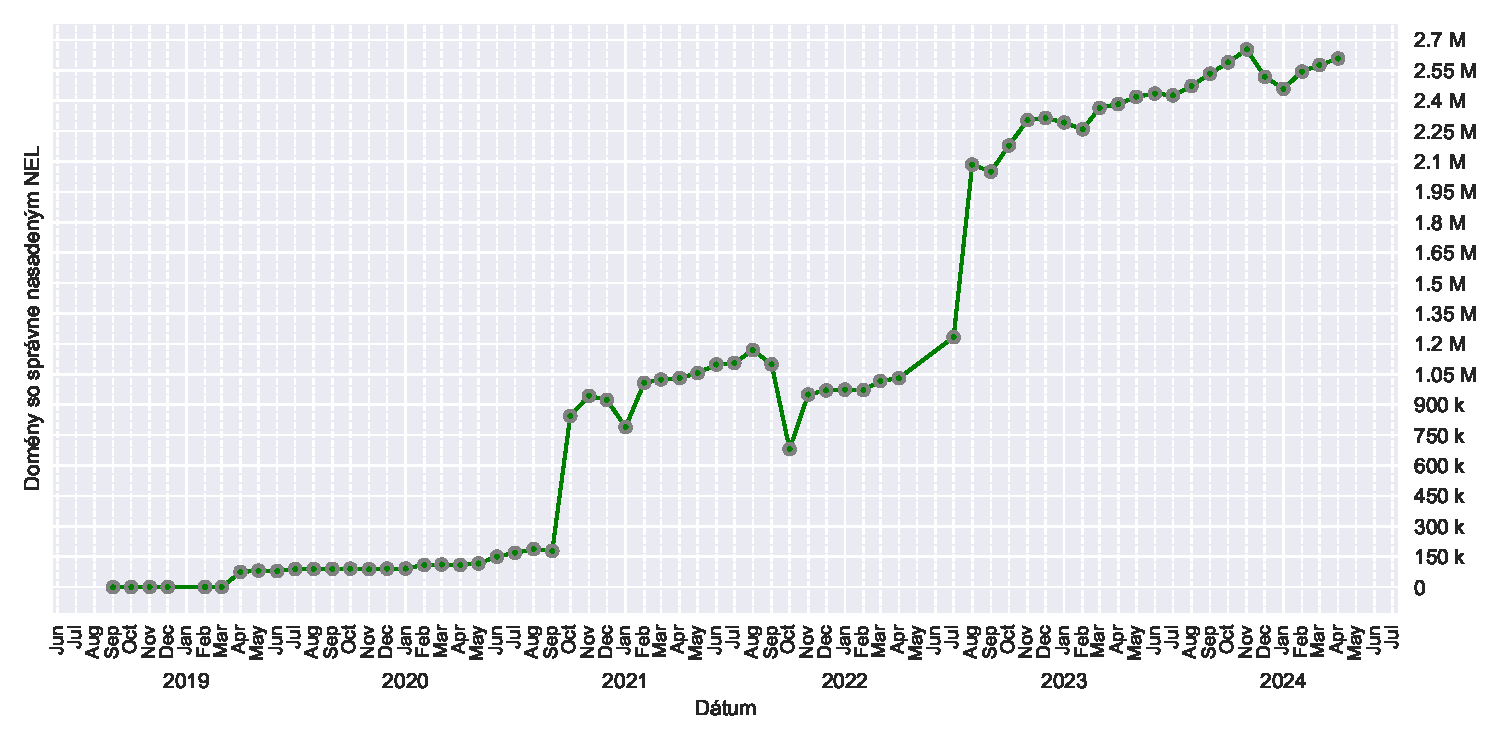
\includegraphics[scale=0.59]{obrazky-figures/httparchive_nel_deployment.pdf}
 \caption{Graf zobrazujúci rast počtu domén so správne nasadenou technológiou NEL.}
 \label{fig:httparchive-nel-deployment}
\end{center}
\end{figure}

Pre pohľad na presné počty po jednotlivých mesiacoch som ďalej zhotovil graf uvedený v obrázku \ref{fig:httparchive-nel-deployment_ratio_values}.
Z neho je možné vyčítať doplnkové informácie:
\begin{itemize}
    \item počiatočný počet skúmaných domén bol 2 096 799, 
    \item počet skúmaných domén v poslednom skúmanom mesiaci bol 20 424 419,
    \item počiatočné percentuálne nasadenie NEL bolo 0.000095\%,
    \item percentuálne nasadenie NEL v poslednom skúmanom mesiaci bolo 12.77\%,
    \item presný počet domén pri výrazných nárastoch a poklesoch v nasadení NEL:
    \begin{itemize}
        \item november 2018 -- nárast z 10 domén na 187,
        \item apríl 2019 -- nárast z 382 domén na 74 590,
        \item október 2020 -- nárast z 178 670 domén na 844 665,
        \item január 2021 -- pokles z 923 400 domén na 789 667,
        \item október 2021 -- pokles z 1 099 507 domén na 680 909,
        \item august 2022 -- nárast z 1 233 049 domén na 2 084 724,
        \item december 2023 -- pokles z 2 653 529 domén na 2 518 117.
    \end{itemize}
\end{itemize}

Na tomto grafe, tak ako aj na niekoľkých ďalších, sa prejavil výpadok dát za mesiace máj a jún v roku 2022.
Pre tie mesiace platí, že žiadne NEL domény v dátach HTTP Archive jednoducho nájdené neboli. 
To platí zároveň pre všetky ostatné mesiace, ku ktorým prislúcha iba číslo 0.

\begin{figure}[!htb]
\begin{center}
 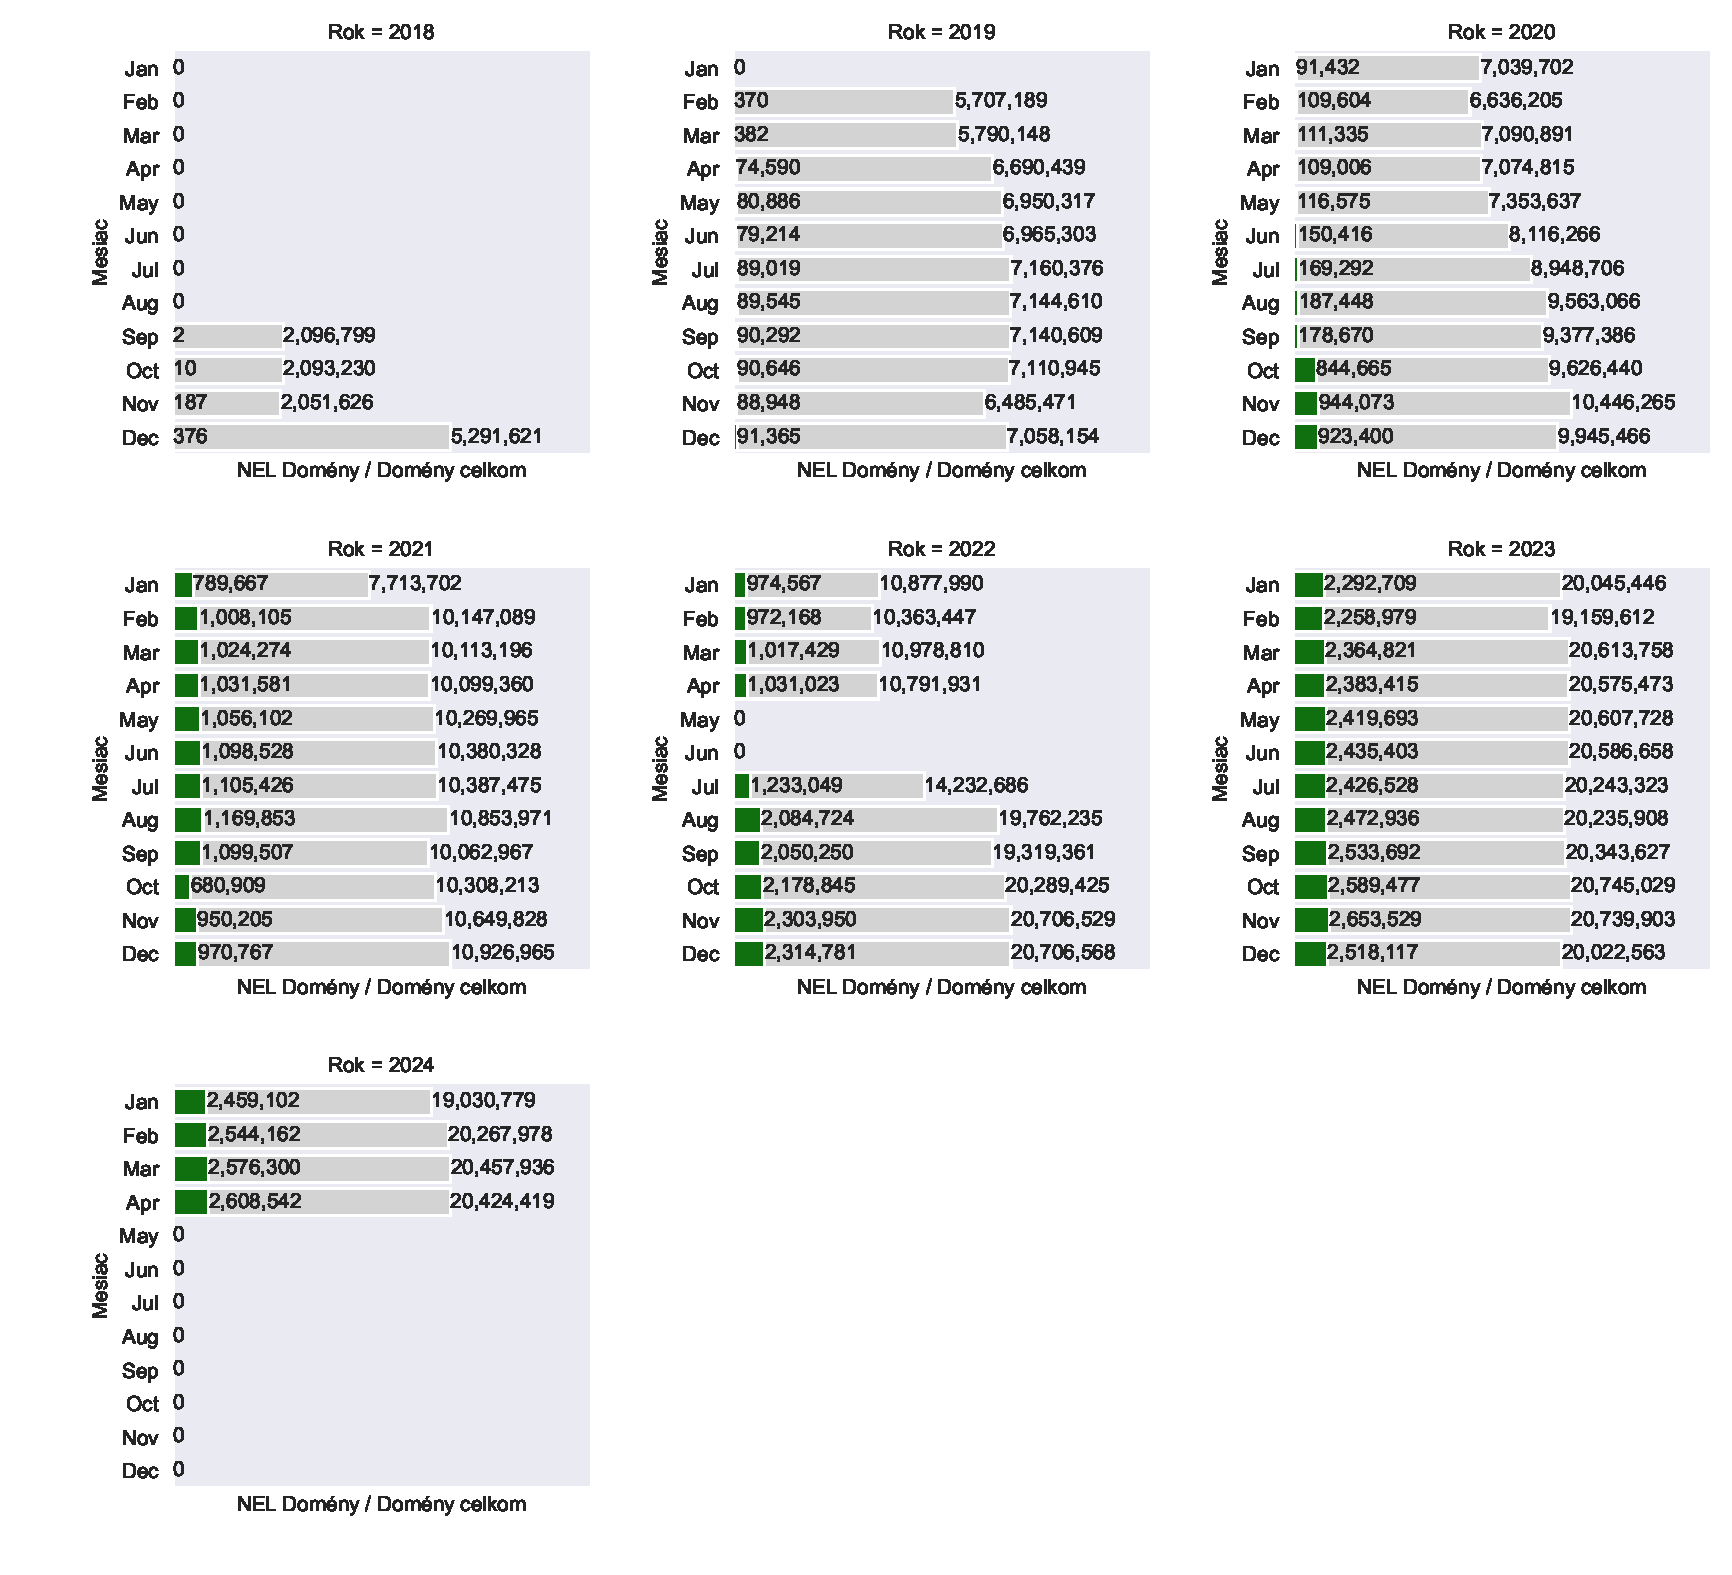
\includegraphics[scale=0.518]{obrazky-figures/httparchive_nel_deployment_ratio_values.pdf}
 \caption{Graf zobrazujúci presné počty domén so správne nasadenou technológiou NELs v porovnaní s celkovým počtom preskúmaných domén za jednotlivé mesiace.}
 \label{fig:httparchive-nel-deployment_ratio_values}
\end{center}
\end{figure}

\pagebreak


\subsubsection{Poskytovatelia používaných NEL kolektorov}

% TODO definovať v teórií poskytovateľa kolektorov
Počet poskytovateľov NEL kolektorov používaných počas skúmaného obdobia je pomerne malý.
Identifikoval som 425 poskytovateľov, ktoré sa za toto obdobie vyskytli.
Počet aktívnych poskytovateľov po jednotlivých mesiacoch uvádza graf v obrázku \ref{fig:httparchive-nel-collector-provider-count}.
Graf vykresľuje stabilný, postupný nárast v ich počte.
Počas tohto rastu dvakrát došlo k výraznému poklesu.
Prvý v júli 2022, hneď po výpadku HTTP Archive dát.
Druhý neskôr v marci 2023.

Z výsledných dát vypočítanej metriky pre kolektory viem, že prvým poskytovateľom NEL kolektorov bola doména \code{bingparachute.com}.
Počiatočne ho používali práve 2 jedinečné domény.
Za posledný preskúmaný mesiac bolo aktívnych presne 326 poskytovateľov.

\begin{figure}[!htb]
\begin{center}
 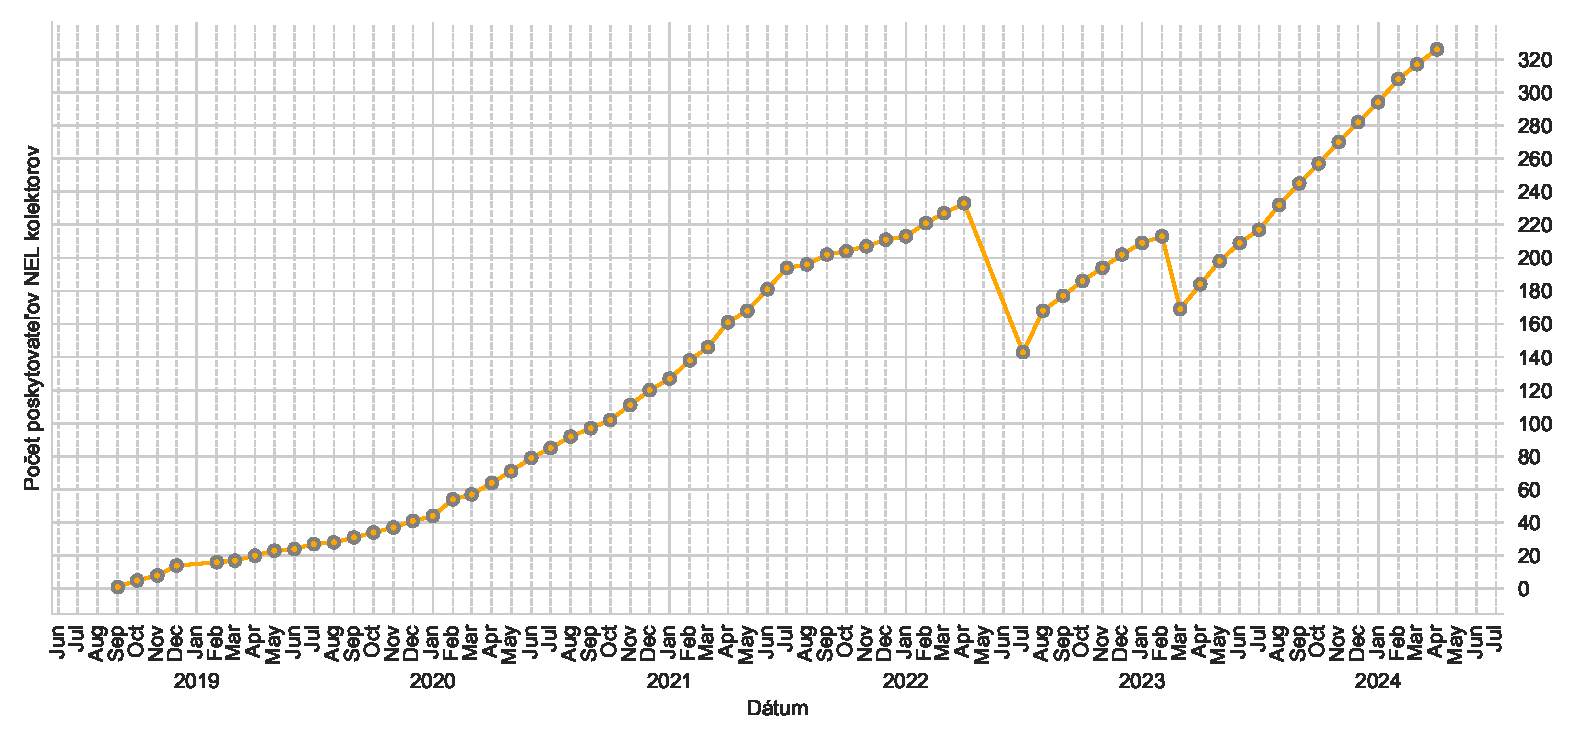
\includegraphics[scale=0.57]{obrazky-figures/httparchive_nel_collector_provider_count.pdf}
 \caption{Graf zobrazujúci rast počtu poskytovateľov NEL kolektorov.}
 \label{fig:httparchive-nel-collector-provider-count}
\end{center}
\end{figure}

\pagebreak

Vizualizácia v obrázku \ref{fig:httparchive-nel-collector-provider-top-1-over-time} zobrazuje poskytovateľov NEL kolektorov s najvyšším počtom obsluhovaných domén za skúmané obdobie. 
Vďaka tomuto grafu som zistil, že tie najviac badateľné nárasty v počte domén využívajúcich NEL sú spojené s príchodom konkrétnych poskytovateľov NEL kolektorov:
\begin{itemize}
\item november 2018 -- nárast spôsobený kolektormi od \code{report-uri.com},
\item apríl 2019 -- nárast spôsobený kolektormi od \code{shopifycloud.com},
\item október 2020 -- nárast spôsobený kolektormi od \code{cloudflare.com},
\item august 2022 -- nemožno určiť podľa obrázka \ref{fig:httparchive-nel-collector-provider-top-1-over-time}.
\end{itemize}

\begin{figure}[!htb]
\begin{center}
 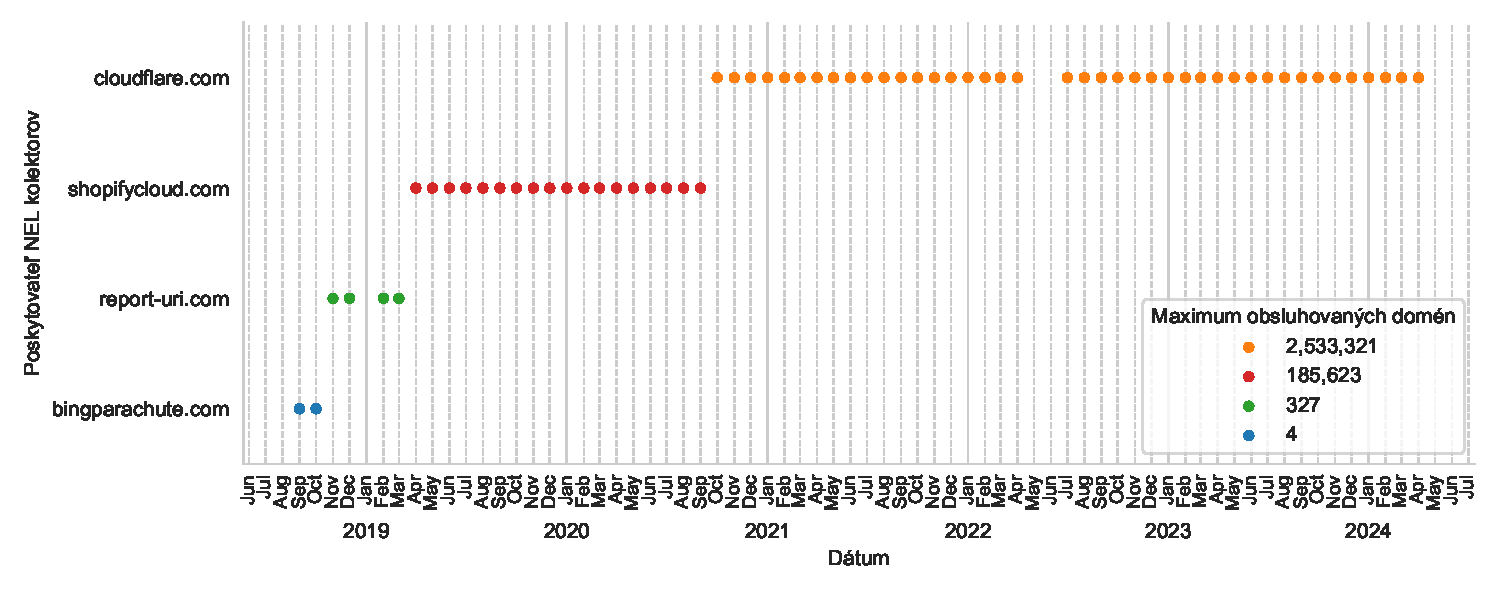
\includegraphics[scale=0.598]{obrazky-figures/httparchive_nel_collector_provider_top_1_over_time.pdf}
 \caption{Poskytovatelia NEL kolektorov s najvyšším počtom obsluhovaných domén pre každý skúmaný mesiac. }
 \label{fig:httparchive-nel-collector-provider-top-1-over-time}
\end{center}
\end{figure}

\pagebreak

Nárast za august 2022 však môžem popísať dátami z použitej metriky pre graf v obrázku vyššie.
O tento nárast sa prevažne zaslúžil \code{cloudflare.com}, najpoužívanejší poskytovateľ NEL kolektorov v tom čase. 
Počet ním obsluhovaných domén totiž z júna 2022 na august 2022 narástol o 836 324.

\subsubsection{História hlavných poskytovateľov NEL kolektorov}

Okrem iného je zo získaných dát možné preskúmať poskytovateľov NEL kolektorov do hĺbky.
Pre rozsahové limity tejto práce som si na ukážku musel nejakým spôsobom vybrať množinu poskytovateľov na hlbší prieskum.
Cieľom bolo vybrať tých čo najviac relevantných.
Z dát som zistil, že sa pre každý mesiac v skúmanom období vyskytoval práve jeden značne dominantný poskytovateľ v počte obsluhovaných domén.
V prevažnej väčšine mesiacov je pomer obsluhy domén dominantným poskytovateľom k celkovej obsluhe všetkými dostupnými poskytovateľmi viac ako 90\%.
Týchto dominantných poskytovateľov už popisuje graf v obrázku \ref{fig:httparchive-nel-collector-provider-top-1-over-time} vyššie.

Ako zaujímavých som si nakoniec vybral najpoužívanejších 10 poskytovateľov za posledný mesiac v skúmanom období.
Zahŕňajú jednak toho najdominantnejšieho poskytovateľa za celé skúmané obdobie, ale aj niektorých, čo poskytujú svoje kolektory už od roku 2020 a skôr.
Znázorňuje ich tabuľka \ref{tab:top-10-latest-nel-collector-providers-stats}.

Zistil som, že iba \code{cloudflare.com} začal testovať NEL na iba jedinej obsluhovanej doméne. Naopak, maximum domén obsluhovaných v mesiaci nasadenia dosahuje \code{fandom.com}.
Poskytovateľ, ktorý sa v rámci tejto množiny objavil ako prvý je \code{report-uri.com}.
Poskytuje totiž NEL kolektory už od druhého skúmaného mesiaca za celé obdobie, konkrétne od októbra 2018.
Posledný stĺpec v tabuľke \ref{tab:top-10-latest-nel-collector-providers-stats} potvrdzuje skutočnosť, že \code{cloudflare.com} je naozaj značne dominantným poskytovateľom NEL kolektorov.
Stĺpec totiž obsahuje hodnoty reprezentujúce podiely na obsluhe celkového počtu domén s nasadeným NEL, pričom \code{cloudflare.com} má podiel skoro 96,3\%.

\begin{table}[!htb]
\centering
\resizebox{\textwidth}{!}{\begin{tabular}{ll||r|r|r|rr}
\toprule
Dátum & Poskytovateľ & D. nasadenia & Obsluha (nasadenie) & Obsluha (aktuálne) & \% z celku za mesiac \\
\midrule
\midrule
\multirow{10}{*}{Apr 2024} & cloudflare.com & Aug 2020 & 1 & 2,511,907 & 96.273 \\
& heroku.com & Aug 2023 & 2 & 45,405 & 1.740 \\
& fandom.com & May 2023 & 11 & 29,833 & 1.143 \\
& freshedge.net & Oct 2022 & 5,772 & 8,999 & 0.345 \\
& dz8aopenkvv6s.cloudfront.net & Aug 2022 & 2,552 & 3,829 & 0.147 \\
& wikimedia.org & Sep 2020 & 27 & 1,447 & 0.055 \\
& hhdev.ru & Aug 2021 & 120 & 1,385 & 0.053 \\
& report-uri.com & Oct 2018 & 3 & 1,190 & 0.046 \\
& yandex.net & May 2020 & 19 & 1,082 & 0.041 \\
& gumlytics.com & Dec 2021 & 7 & 610 & 0.023 \\
\bottomrule
\end{tabular}}
\caption{Detaily pre 10 najpoužívanejších poskytovateľov NEL kolektorov za apríl 2024.}
\label{tab:top-10-latest-nel-collector-providers-stats}
\end{table}

Ďalej v obrázku \ref{fig:httparchive-nel-latest-collector-provider-stats} uvádzam graf vizualizujúci približné počty mesačne obsluhovaných domén týmito poskytovateľmi. 
Z grafu je možné vyčítať ako sa od prvého mesiaca funkčnosti daného poskytovateľa menil počet domén, ktoré obsluhuje.
V mesiacoch máj a jún 2022 sa nejedná o prerušenie dostupnosti jednotlivých poskytovateľov, ale o zmienenú absenciu NEL hlavičiek v HTTP Archive dátach.

\begin{figure}[!htb]
\begin{center}
 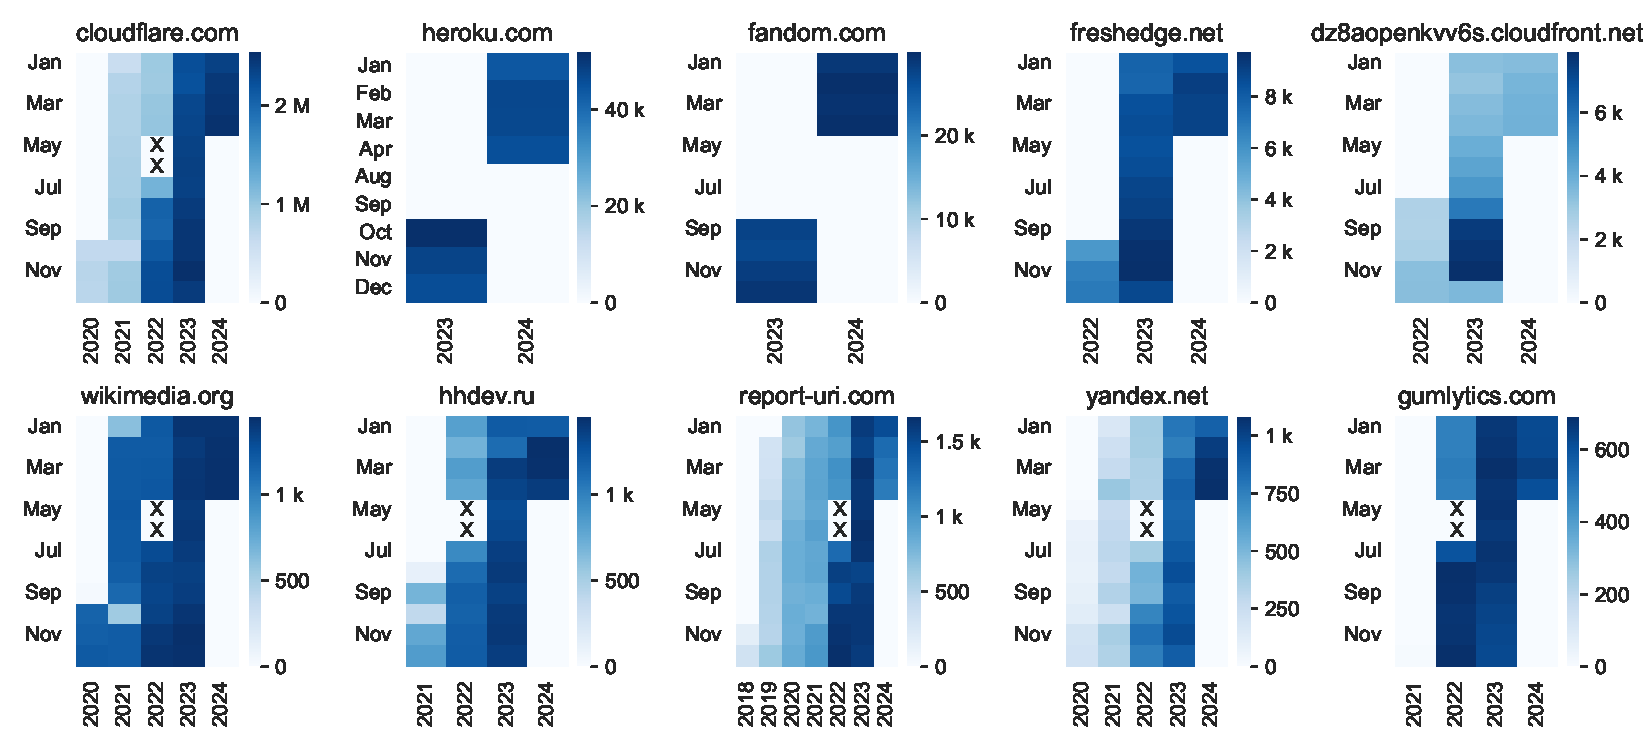
\includegraphics[scale=0.54]{obrazky-figures/httparchive_nel_latest_collector_provider_stats.pdf}
 \caption{Vývin v počte obsluhovaných domén pre 10 najpoužívanejších poskytovateľov NEL kolektorov za apríl 2024.}
 \label{fig:httparchive-nel-latest-collector-provider-stats}
\end{center}
\end{figure}

\pagebreak

\subsubsection{Konfigurácie}

Konfigurácia NEL pozostáva z nastavenia hodnôt pre štyri polia HTTP hlavičky \code{NEL}. Ide o \code{include\_subdomains}, \code{failure\_fraction}, \code{success\_fraction} a \code{max\_age}.

Na základe toho som zhotovil grafy, ktoré sledujú rôzne hodnoty týchto polí počas skúmaného obdobia.

Prvý graf v obrázku \ref{fig:httparchive-nel-config-is-dist} reprezentuje nastavenie poľa \code{include\_subdomains}.
Hodnota \code{true} pre toto pole prevládala od počiatku využívania NEL až do marca 2019.
Odvtedy jednoznačne začala prevládať hodnota \code{false}.
Graf na ose Y vykresľuje hodnoty v logaritmickej škále.

\begin{figure}[!htb]
\begin{center}
 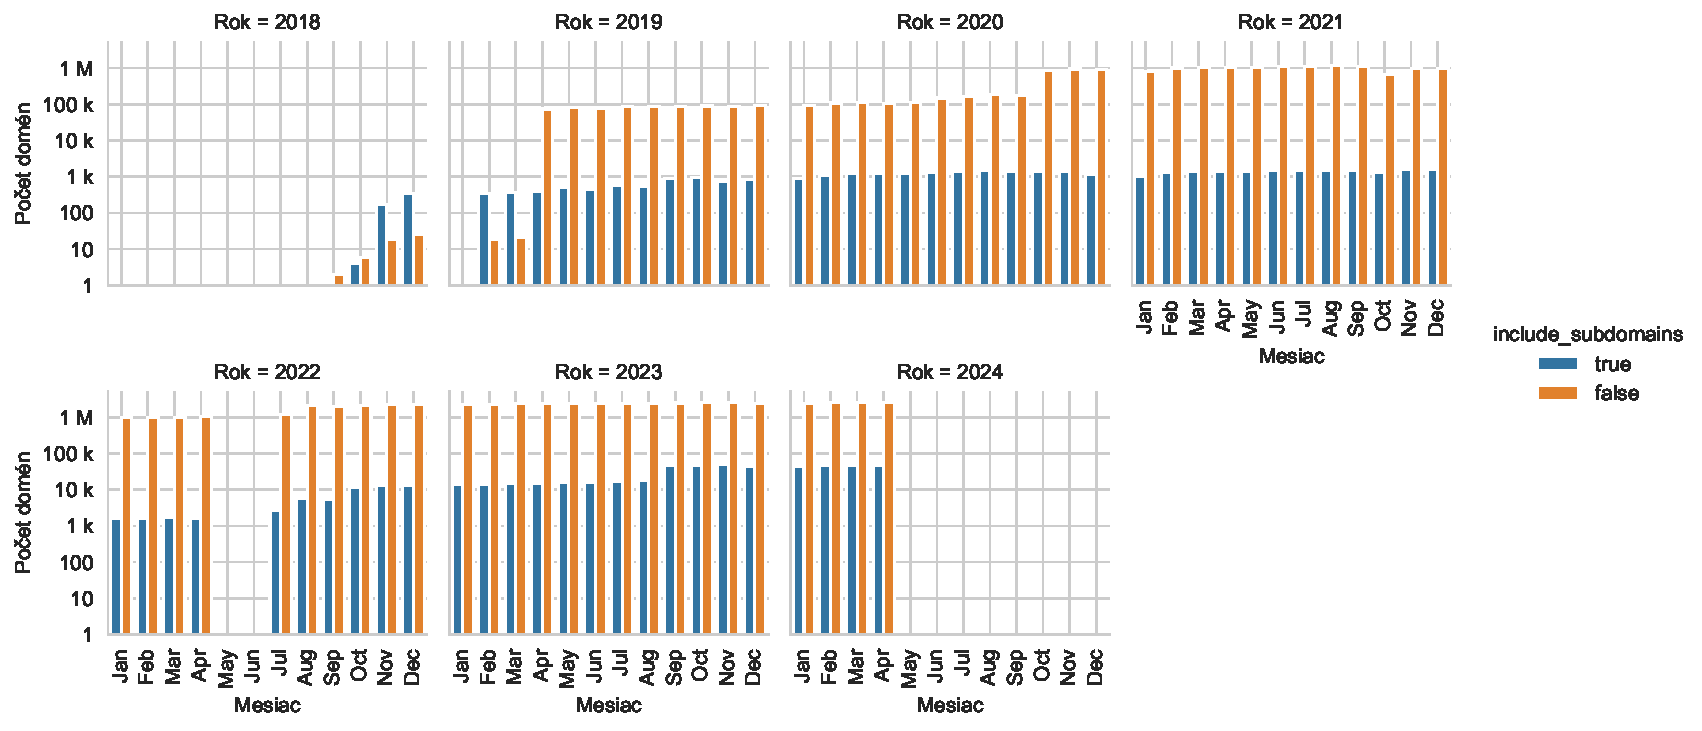
\includegraphics[scale=0.525]{obrazky-figures/httparchive_nel_config_is_dist.pdf}
 \caption{Hodnoty konfiguračného poľa \code{include\_subdomains} počas skúmaného obdobia.}
 \label{fig:httparchive-nel-config-is-dist}
\end{center}
\end{figure}

\pagebreak

Hodnotami pre zvyšné konfiguračné polia sú reprezentácie čísel.
Pre prezentovanie týchto hodnôt som ich rozdelil do intervalov.
Hraničné hodnoty jednotlivých intervalov som zvolil tak, aby reprezentovali často používané hodnoty pre dané konfiguračné pole.

Graf pre pole \code{failure\_fraction} uvádza obrázok \ref{fig:httparchive-nel-config-ff-dist}.
Jednoznačne najviac používaná hodnota tohto poľa je \code{1.0}.
To však platí až od druhej polovice roku 2020. 
Do tej doby bolo najpoužívanejšou hodnotou \code{0.01}.
Naopak, hodnoty v rozmedzí od \code{0.05} až \code{0.10} neboli používané nikdy a hodnota \code{0.00} sa za celý čas vyskytla iba raz.

\begin{figure}[!htb]
\begin{center}
 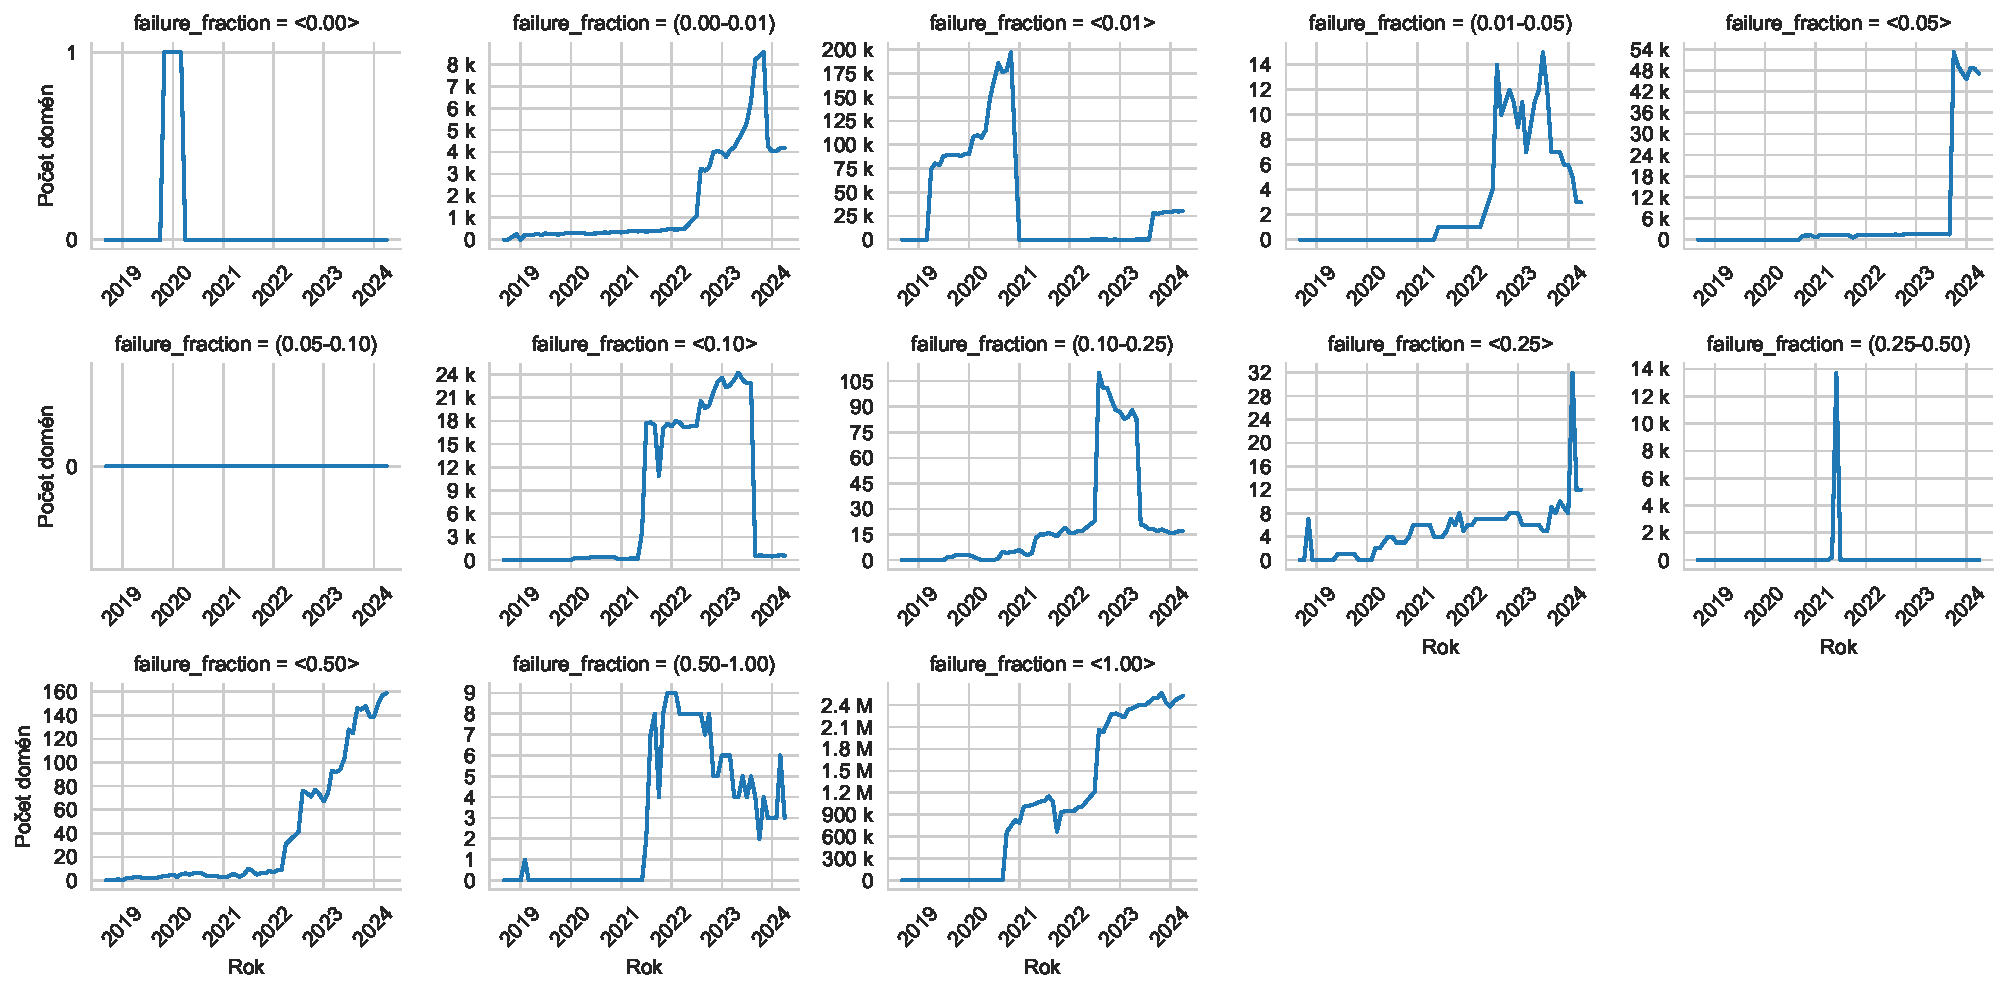
\includegraphics[scale=0.447]{obrazky-figures/httparchive_nel_config_ff_dist.pdf}
 \caption{Hodnoty konfiguračného poľa \code{failure\_fraction} počas skúmaného obdobia.}
 \label{fig:httparchive-nel-config-ff-dist}
\end{center}
\end{figure}

Graf pre ďalšie pole, \code{success\_fraction} je v obrázku \ref{fig:httparchive-nel-config-sf-dist}. 
Prevláda tu hodnota \code{0.00}.

\begin{figure}[!htb]
\begin{center}
 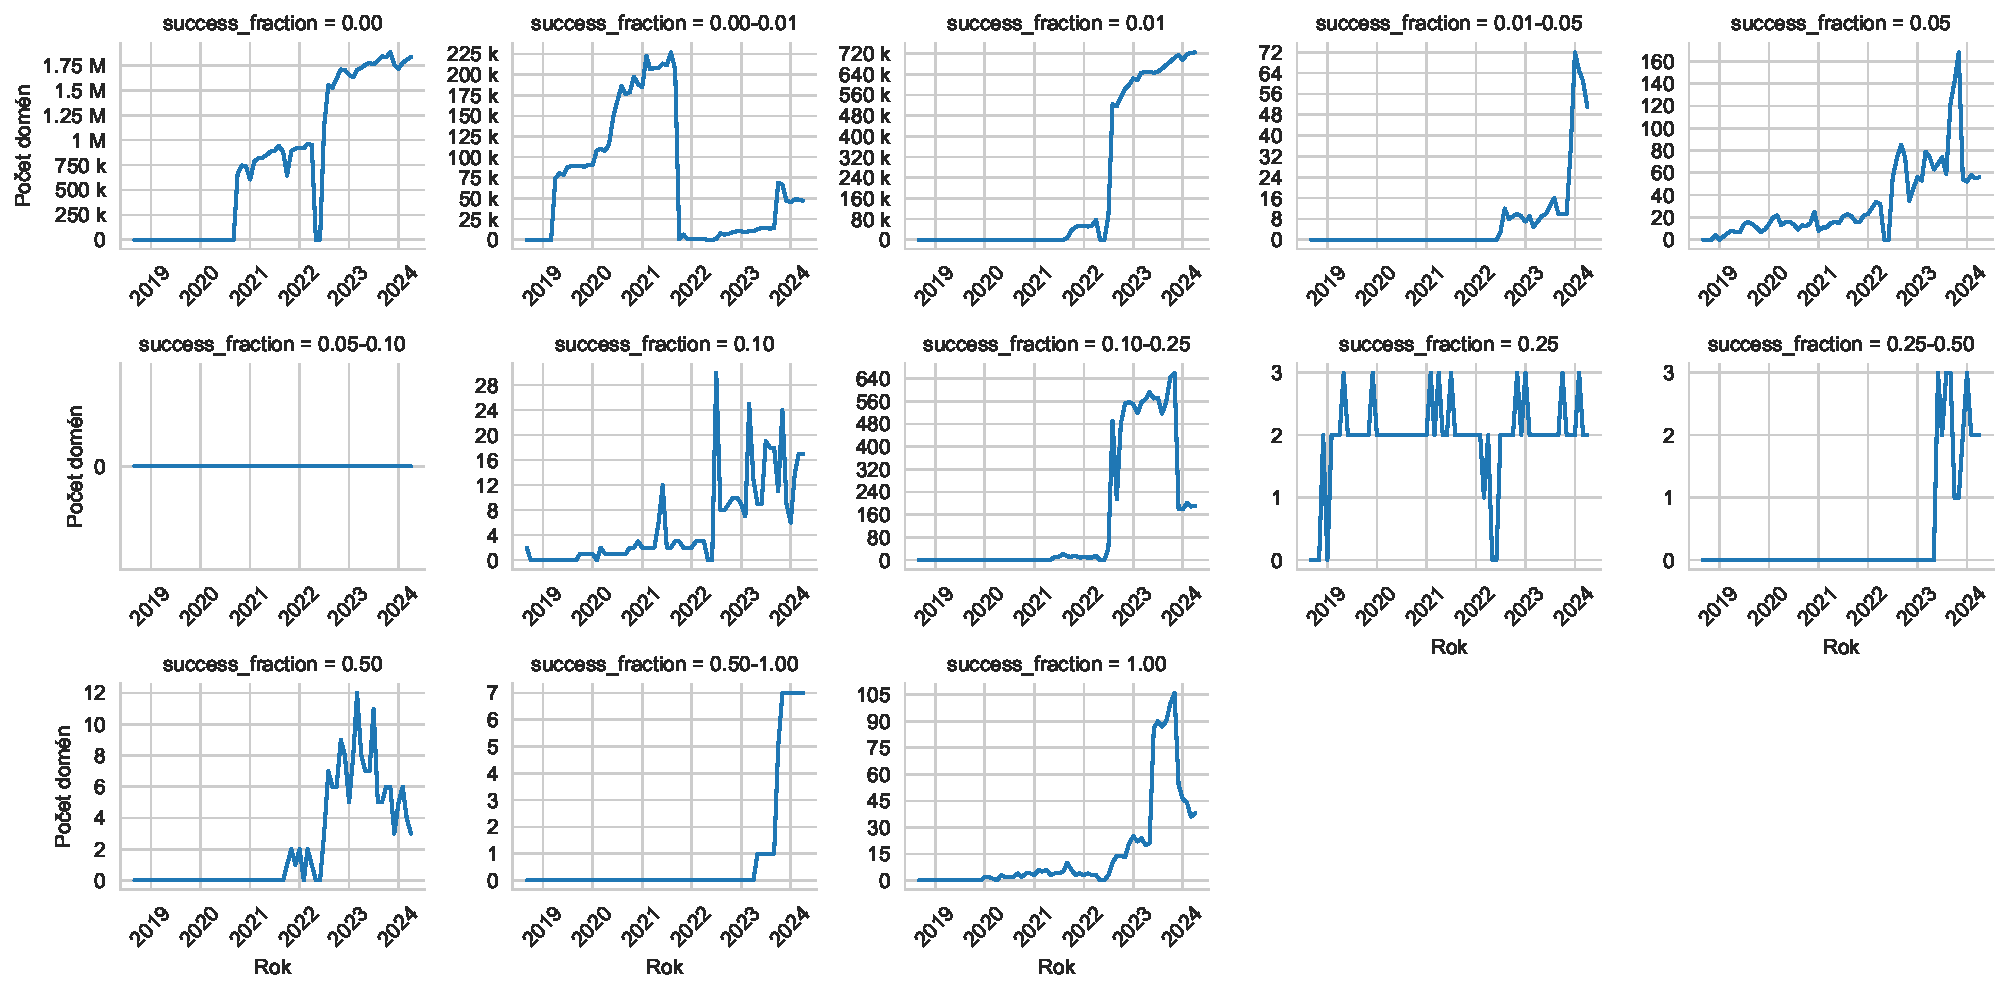
\includegraphics[scale=0.447]{obrazky-figures/httparchive_nel_config_sf_dist.pdf}
 \caption{Hodnoty konfiguračného poľa \code{success\_fraction} počas skúmaného obdobia.}
 \label{fig:httparchive-nel-config-sf-dist}
\end{center}
\end{figure}

\pagebreak

Okrem najčastejšej hodnoty je najzastúpenejšou voľbou \code{0.01}, alebo hodnoty v rozmedzí od \code{0.00} do \code{0.01}.
Zvyšné intervaly hodnôt sa nepoužívajú skoro vôbec.

Posledné pole, \code{max\_age} popisuje graf v obrázku \ref{fig:httparchive-nel-config-ma-dist}.
Prevládajú nastavenia na hodnoty \code{604800}, teda 7 dní v sekundách, alebo \code{2592000}, čo predstavuje 30 dní v sekundách.

\begin{figure}[!htb]
\begin{center}
 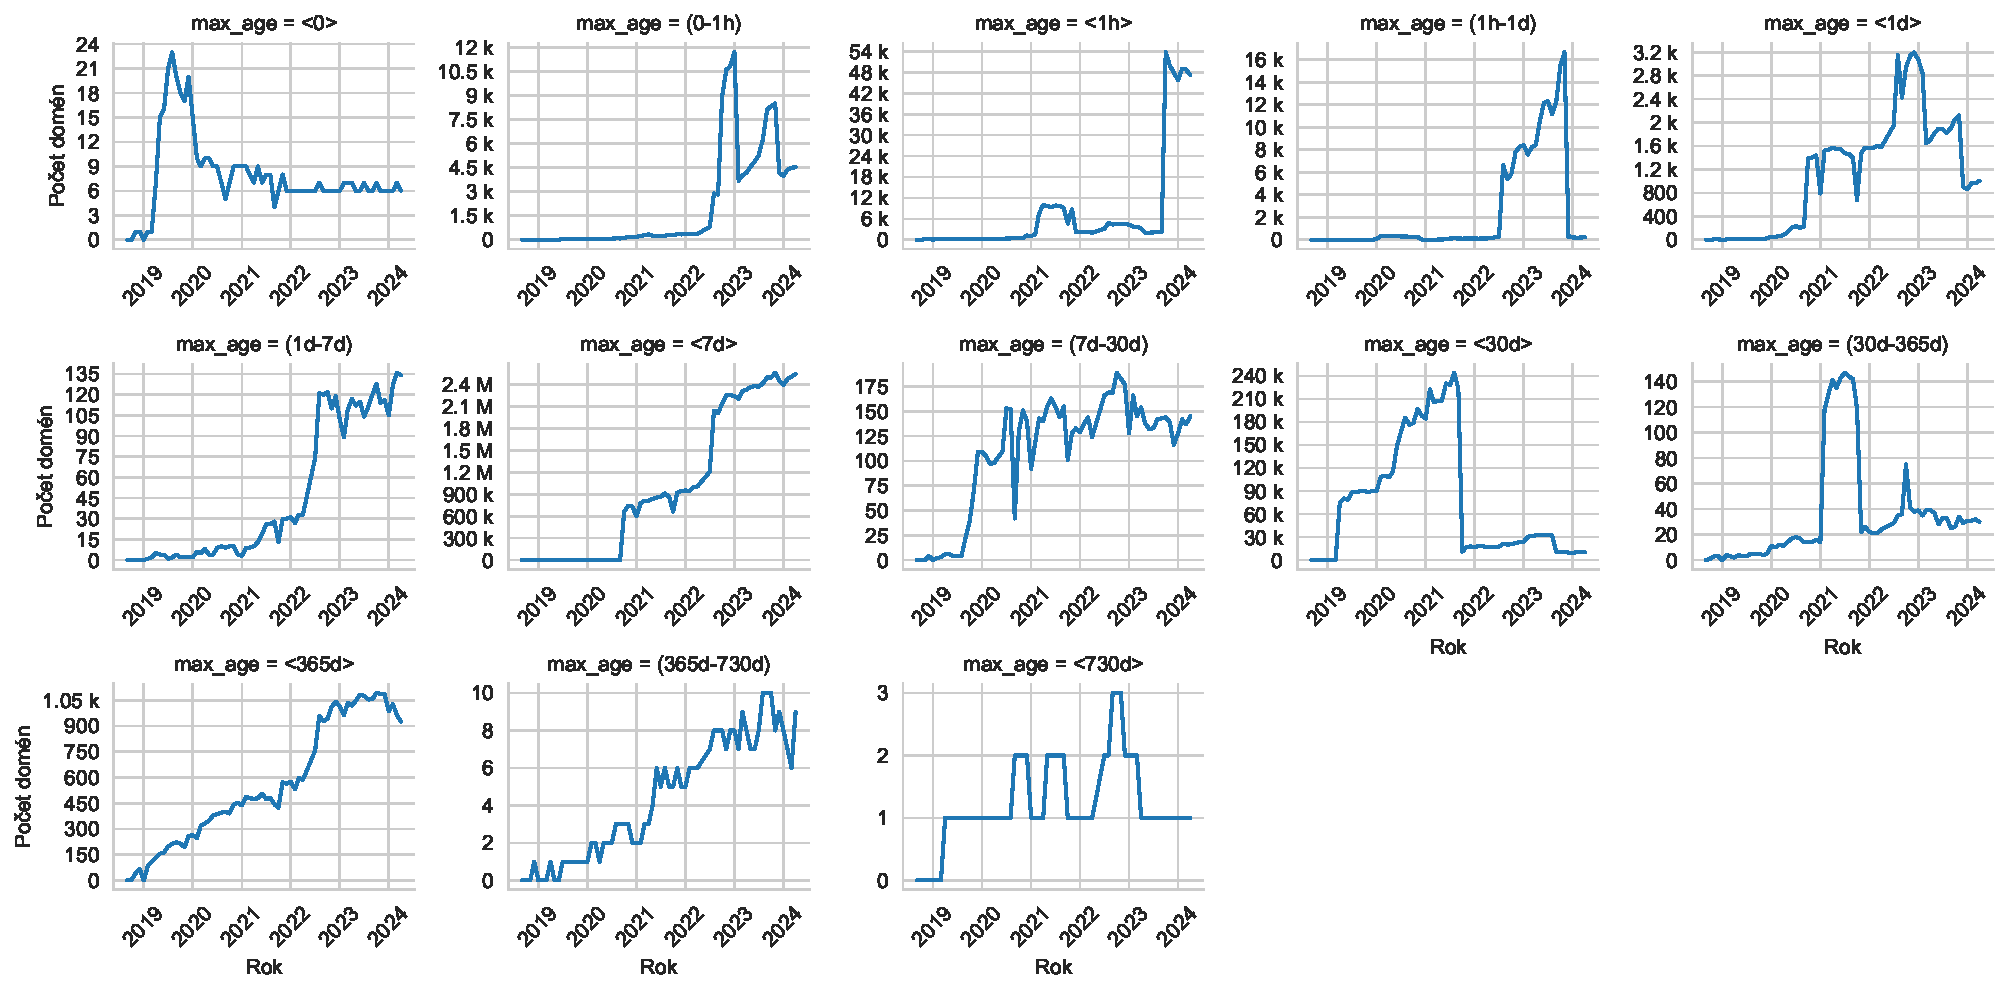
\includegraphics[scale=0.447]{obrazky-figures/httparchive_nel_config_ma_dist.pdf}
 \caption{Hodnoty konfiguračného poľa \code{max\_age} počas skúmaného obdobia.}
 \label{fig:httparchive-nel-config-ma-dist}
\end{center}
\end{figure}

Okrem používanosti samostatných hodnôt som zistil aj aké nastavenia celkovej konfigurácie prevažovali za jednotlivé mesiace.
V tabuľke \ref{tab:nel_config_popular_annual_config} uvádzam najviac vyskytujúce sa variácie konfigurácie NEL za vybrané mesiace.
Pre túto tabuľku som si vybral koniec každého roka a ako posledný riadok som pridal aj posledný mesiac skúmaného obdobia, apríl 2024.
Podľa predošlých grafov je z tejto tabuľky možné vyčítať, že sa s jednoznačnou prevahou používajú v každom zvolenom mesiaci tie najpoužívanejšie hodnoty samostatných polí z daného obdobia.

\begin{table}[!htb]
\centering
% \resizebox{\textwidth}{!}{
\begin{tabular}{l||r|r|r|r|r}
\toprule
Dátum & IS & FF & SF & MA & Počet domén \\
\midrule
\midrule
Dec 2018 & true & 0.00001 & 0.0 & 3600 & 249 \\
Dec 2019 & false & 0.01 & 0.0001 & 2592000 & 90,373 \\
Dec 2020 & false & 1.0 & 0.0 & 604800 & 732,284 \\
Dec 2021 & false & 1.0 & 0.0 & 604800 & 894,283 \\
Dec 2022 & false & 1.0 & 0.0 & 604800 & 1,680,300 \\
Dec 2023 & false & 1.0 & 0.0 & 604800 & 1,732,435 \\
Apr 2024 & false & 1.0 & 0.0 & 604800 & 1,811,335 \\
\bottomrule
\end{tabular}
% }
\label{tab:nel_config_popular_annual_config}
\caption{Najpoužívanejšie konfigurácie NEL za vybrané mesiace.}
\end{table}


\subsubsection{Monitorovanie zdrojov na jednotlivých doménach}

Každá doména s nasadeným NEL ho používa na to aby monitorovala zdroje na nej uložené.
Celkový počet zdrojov, nad ktorými som vykonal analýzu, je viac ako 140 miliónov.
Graf v obrázku \ref{fig:httparchive-nel-deployment-resources} znázorňuje rast počtu monitorovaných zdrojov na skúmaných doménach počas skúmaného obdobia.

\begin{figure}[!htb]
\begin{center}
 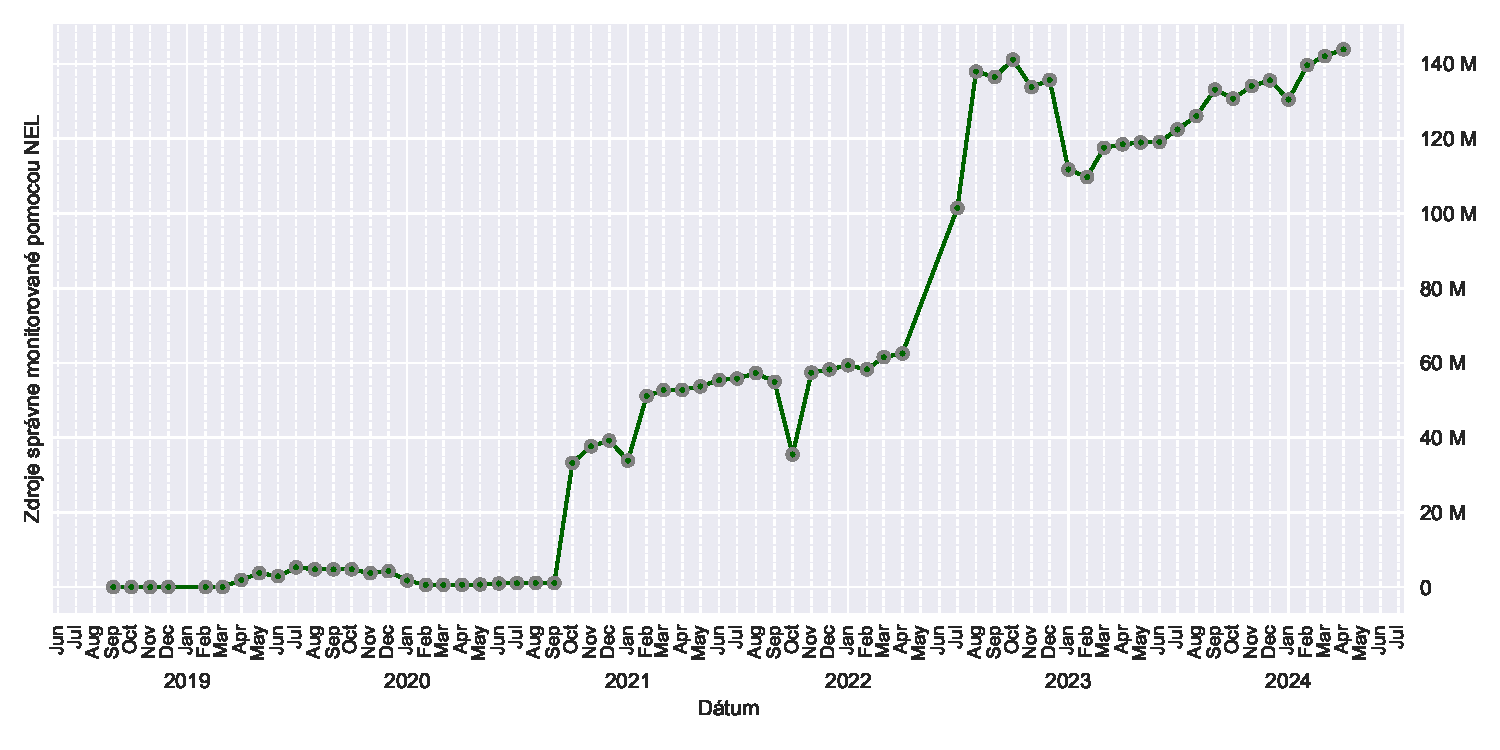
\includegraphics[scale=0.59]{obrazky-figures/httparchive_nel_deployment_resources.pdf}
 \caption{Graf zobrazujúci rast počtu monitorovaných zdrojov na doménach so správne nasadenou technológiou NEL.}
 \label{fig:httparchive-nel-deployment-resources}
\end{center}
\end{figure}

Pri zdrojoch dostupných na jednotlivých doménach som sa zameral na zistenie pomeru počtu monitorovaných zdrojov k celkovému počtu zdrojov dostupných na danej doméne.
Moje zistenia znázorňuje obrázok \ref{fig:httparchive-nel-monitored-resources-precentage-dist} --- prevažná väčšina domén monitoruje všetky zdroje.

\begin{figure}[!htb]
\begin{center}
 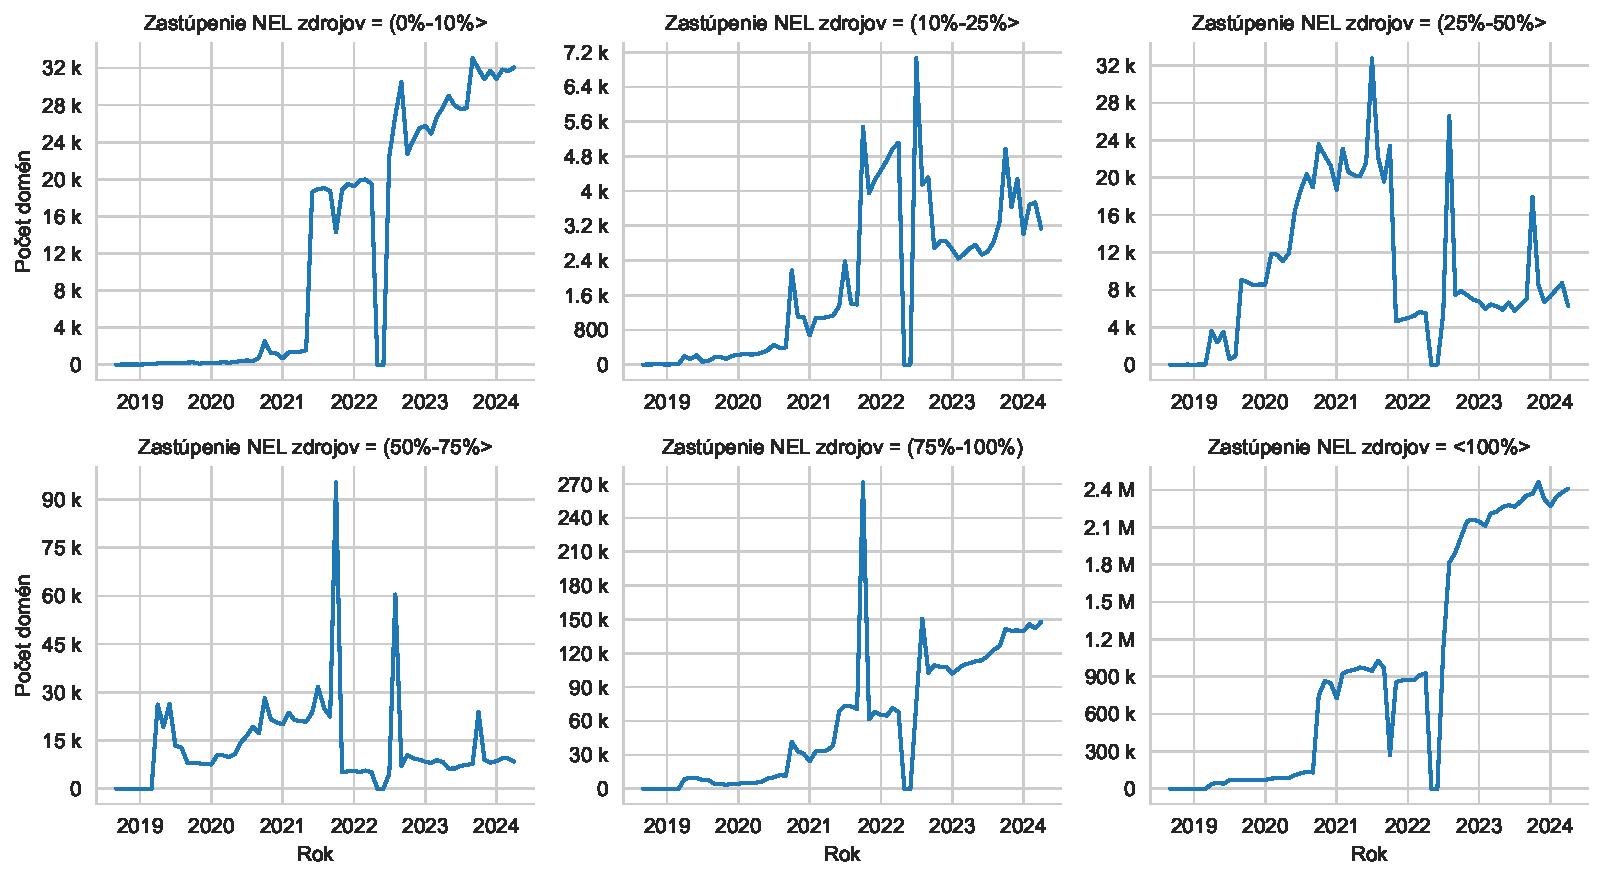
\includegraphics[scale=0.56]{obrazky-figures/httparchive_nel_monitored_resources_percentage_dist.pdf}
 \caption{Počty domén s nasadeným NEL podľa percenta monitorovaných zdrojov.}
 \label{fig:httparchive-nel-monitored-resources-precentage-dist}
\end{center}
\end{figure}

\subsubsection{Detekcia rôznych konfigurácií na skúmaných doménach}

Vďaka tomu, že sú v dátach záznamy pre každý monitorovaný zdroj dostupný na danej doméne, je možné tiež preskúmať, či doména využíva jednu, alebo viac variácií konfigurácie NEL.
Rozhodol som sa teda uviezť ako príklad zistenia za niektoré mesiace.
Vybral som znova posledný mesiac za každý rok, pričom som tiež pridal aj posledný preskúmaný mesiac, apríl 2024.
Zistenia prezentujem v tabuľke \ref{tab:nel-config-variations}.
Najviac zastúpené sú prípady, kde dané domény používajú iba jednu konfiguráciu pre všetky svoje zdroje.
Avšak, naprieč skúmaným obdobím som identifikoval značný počet domén, ktoré používali aspoň dve rôzne konfigurácie.
Domén, ktoré využívali viac ako dve, bolo veľmi málo.
Zistil som však, že maximálny počet rozdielnych NEL konfigurácií na jednotlivých doménach bol až 7.

\begin{table}[!htb]
\centering
\resizebox{\textwidth}{!}{\begin{tabular}{l||r|r|r|r|r|r|r}
\toprule
Dátum & Dec 2018 & Dec 2019 & Dec 2020 & Dec 2021 & Dec 2022 & Dec 2023 & Apr 2024 \\
Počet variácií &  &  &  &  &  &  &  \\
\midrule
\midrule
1 & 375 & 91,355 & 899,292 & 970,362 & 2,293,385 & 2,484,009 & 2,574,899 \\
2 & 2 & 16 & 47,796 & 784 & 42,664 & 67,124 & 66,372 \\
3 & 0 & 6 & 615 & 15 & 51 & 1,563 & 1,317 \\
4 & 0 & 0 & 4 & 0 & 12 & 8 & 4 \\
5 & 0 & 0 & 5 & 0 & 80 & 10 & 5 \\
6 & 0 & 0 & 6 & 0 & 6 & 6 & 6 \\
7 & 0 & 0 & 0 & 0 & 14 & 0 & 0 \\
\bottomrule
\end{tabular}}
\caption{Počty domén s rôznym počtom rozdielnych NEL konfigurácií pre vybrané dátumy.}
\label{tab:nel-config-variations}
\end{table}

\subsubsection{Použitie NEL podľa typu monitorovaných zdrojov}

V rámci skúmania zdrojov som tiež preveril, aké bývajú ich typy.
Obrázok \ref{fig:httparchive-nel-resource-types-dist} predstavuje graf rozdelenia počtov zdrojov podľa ich typu.

\begin{figure}[!htb]
\begin{center}
 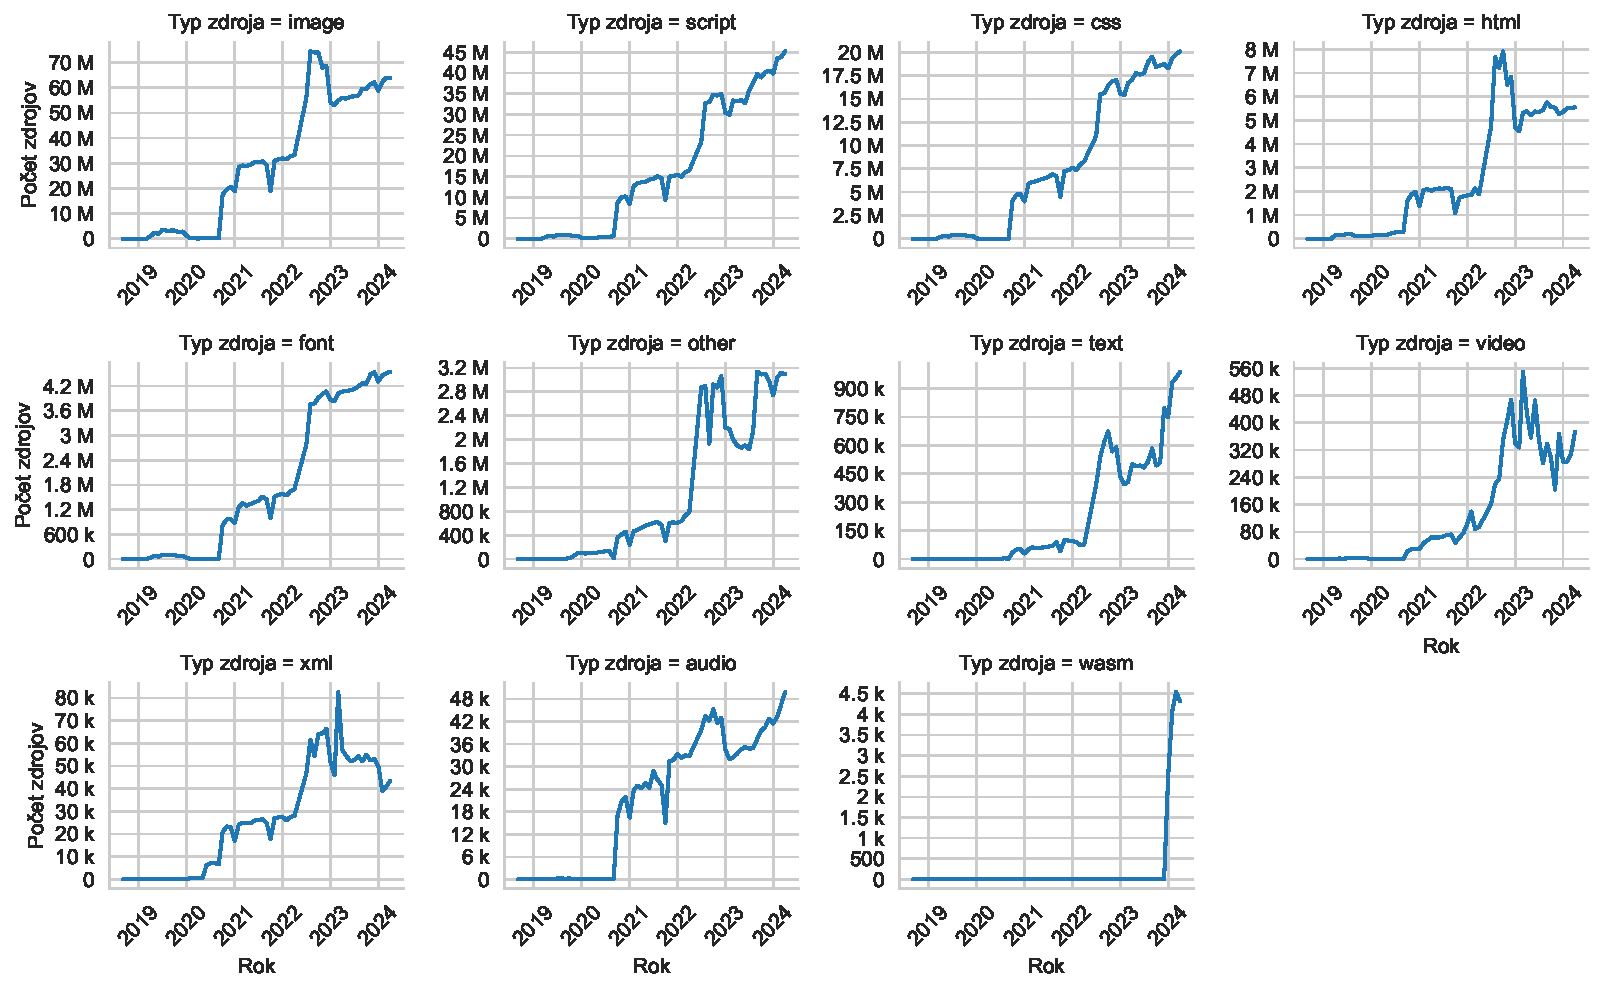
\includegraphics[scale=0.447]{obrazky-figures/httparchive_nel_resource_types_dist.pdf}
 \caption{Počty NEL monitorovaných zdrojov podľa ich typu.}
 \label{fig:httparchive-nel-resource-types-dist}
\end{center}
\end{figure}

Zistil som, že sa NEL využíva najviac na monitorovanie obrázkov, skriptov a kaskádových štýlov CSS.
Toto zistenie však možno doplniť predošlým zistením, že domény zväčša monitorujú všetky svoje zdroje.
Vzhľadom na to som usúdil, že toto skôr poukazuje na skutočnosť, že sa tieto typy zdrojov skrátka vyskytujú najčastejšie.

\subsubsection{Domény s nesprávne nasadeným NEL}

Posledným údajom vypočítaným čisto z dát HTTP Archive je vývin počtu domén s nesprávne nasadeným NEL počas skúmaného obdobia.
Zistil som, že počet týchto domén je zanedbateľný v porovnaní s počtom domén so správne nasadeným NEL.
No dodnes sa stále vyskytujú domény, ktoré v HTTP odpovediach zasielajú hlavičku NEL, ale nejakým spôsobom to vykonávajú nekorektne.
Pri prehliadaní HTTP Archive dát v BigQuery som zistil, že častým prípadom bolo vynechanie HTTP hlavičky \code{Report-To} alebo zle pomenované polia v hlavičke \code{NEL} (napríklad zamenené znaky \code{'\_'} za \code{'-'}). 
Obrázok \ref{fig:httparchive-nel-deployment-incorrect} znázorňuje vývoj v počte domén s nesprávne nasadeným NEL.

\begin{figure}[!htb]
\begin{center}
 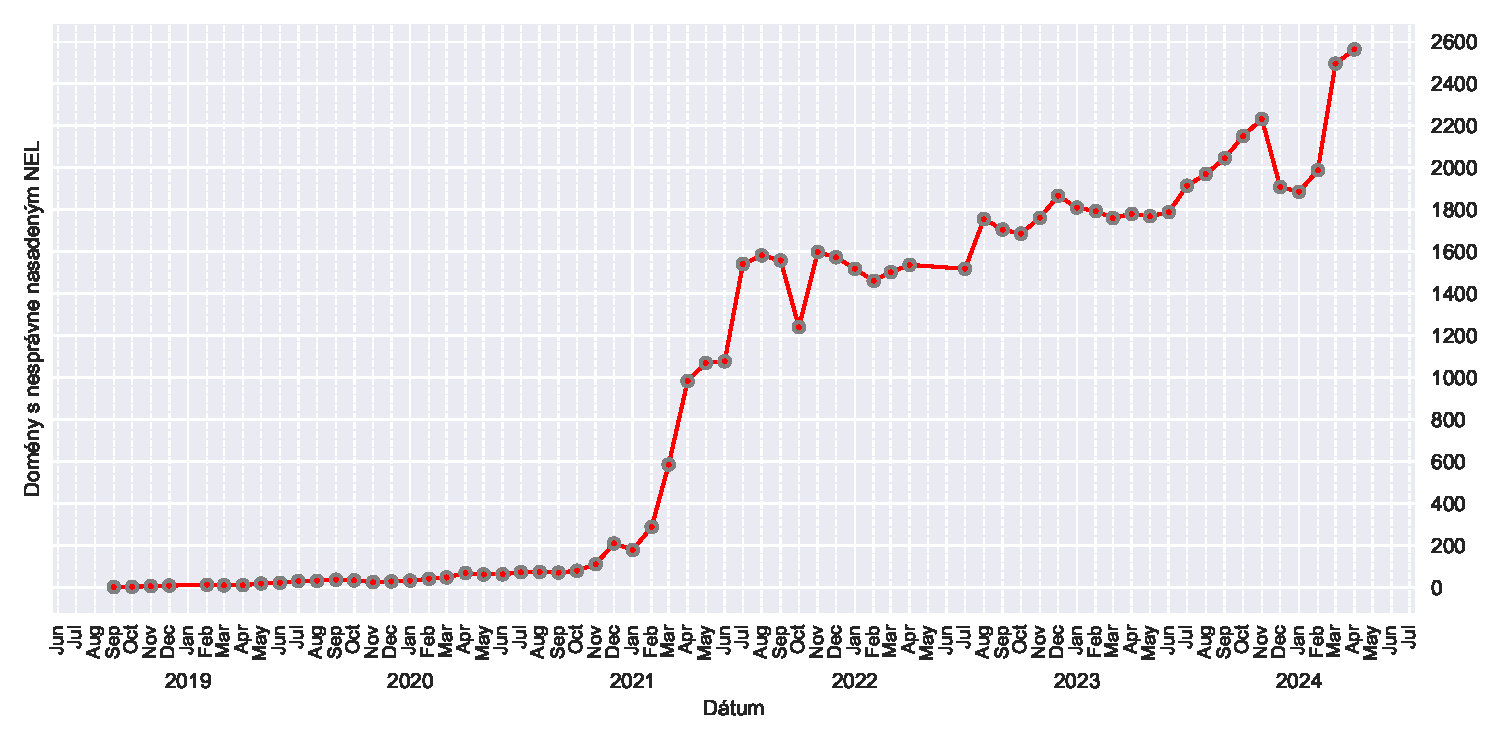
\includegraphics[scale=0.59]{obrazky-figures/httparchive_nel_deployment_incorrect.pdf}
 \caption{Graf zobrazujúci rast počtu domén s nesprávne nasadenou technológiou NEL.}
 \label{fig:httparchive-nel-deployment-incorrect}
\end{center}
\end{figure}


\subsection{Výsledky z automatizovaného prehliadania webu}

Doplnkové dáta z vlastného skriptu na prehliadanie webu sa mi podarilo získať pre 33 070 domén z cieľových 58 596.
Dáta pre zvyšných 25 526 domén som získať nestihol.
Cieľové domény pochádzajú z posledného analyzovaného mesiaca HTTP Archive dát, apríla 2024.
Kritéria pre ich výber boli:
\begin{enumerate}
    \item musia mať dostupných aspoň 20 NEL monitorovaných zdrojov,
    \item musia sa objavovať v rebríčku populárnych domén TRANCO za uvedený mesiac.
\end{enumerate}
Kritéria som vybral tak, aby som mohol skúmať dostatočne veľkú vzorku zdrojov na doméne, pričom by bola šanca, že tam NEL detegujem.
Okrem toho som sa rozhodol použiť tu TRANCO aby som redukoval počet domén na prieskum, pričom ponechám v množine skúmaných tie najviac relevantné.
Zámerom redukcie bolo pracovať iba s takým množstvom domén, ktoré stihnem spracovať skriptom spomínaným v sekcii \ref{crawl_and_store}.

\subsubsection{Domény používajúce NEL}

Z celkového počtu domén, 33 070 sa úspešne podarilo získať dáta iba z 23 183 z nich.
Prehliadanie zvyšných 9 987 domén skončilo chybou alebo presmerovaním na inú doménu. 
Zo všetkých úspešne prehliadaných domén malo správne nasadený NEL 23 083 z nich.
Takže nesprávne nasadený NEL má práve 100 domén a nasadenie NEL je v tomto prípade 99.57\%.
Oproti HTTP Archive dátam je teda pokles v nasadení NEL približne iba 0.43\%.

\subsubsection{Poskytovatelia používaných NEL kolektorov}

Identifikoval som v celku 15 aktívnych poskytovateľov NEL kolektorov.
Dominantným bol jednoznačne \code{cloudflare.com} s podielom 99.25\% na obsluhe celkového počtu domén s nasadeným NEL.
V zozname 10 najpoužívanejších poskytovateľov pre prehliadané domény ostávajú spolu so zmieneným dominantným v nasledujúcom poradí aj:
\begin{itemize}
    \item \code{heroku.com},
    \item \code{yandex.net},
    \item \code{report-uri.com},
    \item \code{hhdev.ru},
    \item \code{wikimedia.org},
    \item \code{dz8aopenkvv6s.cloudfront.net}.
\end{itemize}
Okrem \code{heroku.com}, ktorý obsluhoval 129 domén, každý z poskytovateľov uvedených vyššie obsluhoval menej ako 11 domén.


\subsubsection{Konfigurácie}

Nastavenia NEL prevládajú nasledujúce:
\begin{itemize}
    \item \code{include\_subdomains} = \code{false} (99.90\%),
    \item \code{failure\_fraction} = \code{1.0} (99.36\%),
    \item \code{success\_fraction} = \code{0.0} (94.43\%) alebo \code{0.01} (4.96\%),
    \item \code{max\_age} = \code{604800}, teda 7 dní (99.27\%).
\end{itemize}

\subsubsection{Monitorovanie zdrojov na jednotlivých doménach}

Totálny počet monitorovaných zdrojov na prehliadaných doménach bol 3 962 754.
Oproti počtu úspešne prehliadaných domén, ktorý bol 23 083, je toto číslo nepomerne veľké oproti tomu, aký pomer som našiel v dátach z HTTP Archive.
HTTP Archive dáta totiž obsahovali pre každú doménu priemerne 7 na nej monitorovaných zdrojov.
Vo výstupných dátach z môjho skriptu to bolo priemerne 172 monitorovaných zdrojov pre každú doménu.  
Aj práve táto skutočnosť mohla zapríčiniť to, že sa mi nepodarilo včas dokončiť prehliadanie celkovej množiny vybratých domén. 
Mojim skriptom totiž prehliadam oveľa viac monitorovaných zdrojov v porovnaní s projektom HTTP Archive a prehliadanie teda trvá príliš dlho.

Zistil som však, že najzastúpenejšie pomery monitorovaných zdrojov k celkovému počtu zdrojov sú:
\begin{itemize}
    \item 100\% monitorovanosti zdrojov (85.99\% domén),
    \item od 75\% po 100\% monitorovanosti zdrojov (10.57\% domén),
    \item od 10\% po 25\% monitorovanosti zdrojov (2.70\% domén).
\end{itemize}

\subsubsection{Detekcia rôznych konfigurácií na skúmaných doménach}

Z dát prehliadania sa mi podarilo zistiť, že maximálny počet variácií konfigurácie NEL je tentokrát iba 3.
Aj v tomto prípade ale väčšina domén používa iba jedinú konfiguráciu (takmer 99\%).

\subsubsection{Použitie NEL podľa typu monitorovaných zdrojov}

Výsledky sú pre túto metriku vypočítanú dátami z prehliadania webu mierne odlišné od výsledkov z dát HTTP Archive. 
Dalo sa to však očakávať vzhľadom na už spomínaný fakt, že stratégia prehliadania monitorovaných zdrojov sa pre môj skript a projekt HTTP Archive očividne líši.
Napríklad markantne stúpol počet zdrojov typu \code{html}, pretože môj skript podľa získaných dát prehliada v priemere väčší počet monitorovaných zdrojov na prehliadanej doméne. 
Najzastúpenejšie typy monitorovaných zdrojov boli:
\begin{enumerate}
    \item \code{image} -- 2 457 577 zdrojov,
    \item \code{script} -- 483 698 zdrojov,
    \item \code{html} -- 482 927 zdrojov, pričom došlo k značnému nárastu oproti zdrojom typu \code{css},
    \item \code{css} -- 312 895 zdrojov.
\end{enumerate}


\section{Pokračovanie práce}

Vzhľadom na to, že sa mi v mojej práci podarilo získať všetky dáta, ktoré sú potrebné na podrobnú analýzu využívania technológie NEL, je nepravdepodobné, že sa vyžaduje pokračovanie v získavaní zdrojových dát.
Avšak, určite je možné preskúmať iné, potencionálne lepšie stratégie použiteľné pre skript na automatizované prehliadanie webu, ktorý analýzu môže vykonávať priebežne.
Tiež je pravdepodobné, že v blízkej budúcnosti bude publikovaná nová špecifikácia NEL, ktorá bude fungovať spolu s novšou verziou Reporting API, a teda bude nutné tento skript upraviť.

Ako som už zmienil na konci sekcie \ref{result-data}, všetky získané dáta odovzdávam vedúcemu mojej práce.
Spolu s nimi budú naďalej používané aj mnou implementované nástroje na vykonávanie analýzy za účelom vypracovania vedeckého článku týkajúceho sa využívania technológie NEL. 
